% Meta-monografia de exemplo genérico de uso da classe delaetex.cls
% Copyright (C) 2004..2016 Walter Fetter Lages <fetter@ece.ufrgs.br>
%
% This file was adapted from:
% Meta-monografia de exemplo genérico de uso da classe deletex.cls
% Copyright (C) 2004 Walter Fetter Lages <w.fetter@ieee.org>
%
% This is free software, distributed under the GNU GPL; please take
% a look in `deletex.cls' to see complete information on using, copying
% and redistributing these files
%
%\documentclass[repeatfields,openright,overleaf,nomicrotype]{tcc}
% LTeX: language=pt-BR
\documentclass[repeatfields,xlists,xpacks,oneside,yearsonly]{ufrgscca}

\graphicspath{{./img/}}
\usepackage{fancybox}
\usepackage{subcaption}
\addbibresource{TCC.bib}
\usepackage[]{todonotes}
\setlength{\marginparwidth}{2cm}

\begin{document}

\maketitle

% dedicatória é opcional
%\notoc\chapter{Dedicatória} %não vai aparecer no sumário

% agradecimentos são opcionais
%\notoc\chapter{Agradecimentos}

% Agradeço ao \LaTeX\ por não ter vírus de macro\ldots

% resumo no idioma do documento
\begin{abstract}

\end{abstract}

% resumo no outro idioma
% como parâmetro devem ser passadas as palavras-chave
% no outro idioma, separadas por vírgulas
\begin{otherabstract}{KEYWORDS TRANSLATION PLACEHOLDER}

\end{otherabstract}

% sumario
\setcounter{tocdepth}{3}

% lista de ilustrações
\listoffigures

% lista de tabelas
\listoftables
% lista de listagens (código fonte)
%\listofcodelist %% doesn't work on overleaf

% lista de abreviaturas e siglas
% o parametro deve ser a abreviatura mais longa
\begin{listofabbrv}{PPGEE}
    \item[BT] \textit{Behavior Tree} (árvore de Comportamento)
    \item[RGB-D] \textit{Red Green Blue - Depth} (vermelho verde azul -
    profundidade)
    \item[ROS] \textit{Robot Operating System} (sistema operacional de robôs)
    \item[SLAM] \textit{Simultaneous Localization and Mapping} (localização e
    mapeamento simultâneos)
    \item[UFRGS] Universidade Federal do Rio Grande do Sul
\end{listofabbrv}

% lista de símbolos é opcional
% \begin{listofsymbols}{$\alpha\beta\pi\omega$}
% \end{listofsymbols}

\tableofcontents

\chapter{Introdução}

A robótica deve seu maior sucesso à indústria de manufatura, onde são
utilizados principalmente robôs
manipuladores~\cite{IntroductionToMobileRobots}. Porém, esses robôs
têm como limitação sua mobilidade, incapazes de se movimentar pela
planta, limitando suas tarefas a um espaço fixo. Um robô móvel, por
outro lado, é capaz de se mover pelo seu ambiente de trabalho,
aumentando a gama de tarefas que podem ser realizadas.

O mercado desta categoria de robô está em crescimento, como mostra a
Figura~\ref{fig:mercado_robo}. Estes robôs podem ser utilizados em
ambientes internos, como hospitais, fábricas ou em centros de
distribuição, como o robô Proteus, da Amazon~\cite{amazon_robot}.
Eles tem como desafio a navegação em ambientes dinâmicos, muitas
vezes compartilhados com humanos. Portanto, é necessária a capacidade
de perceber seu ambiente e replanejar sua trajetória em tempo real,
de modo a evitar colisões. \todo[inline]{Laranja disse que esta parte
    ficou meio enrolada}

\begin{figure}[htbp]
    {
        \centering
        \caption{Mercado global de robôs autônomos de 2016 a 2021, com projeção até 2028.}
        \label{fig:mercado_robo}
        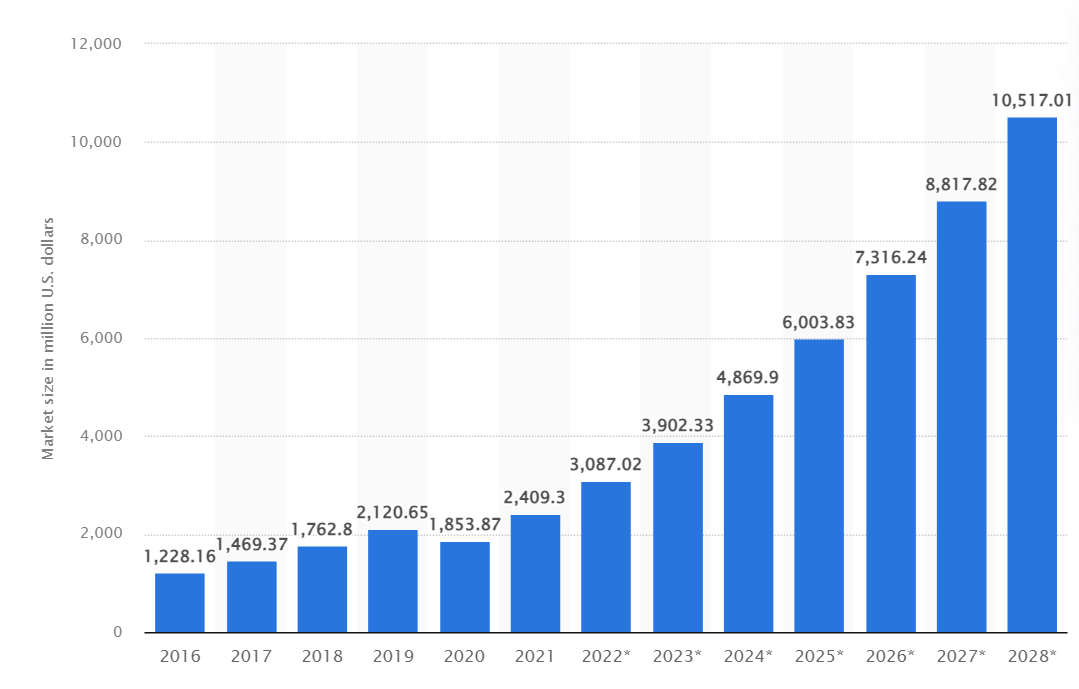
\includegraphics[width=0.75\textwidth]{mercado_robo}\\
    }
    {\sourcecitation{\textcite{robot_market}.}}
\end{figure}

É neste contexto que se insere o projeto atual.
Utilizando o robô Twil, representado na Figura \ref{fig:robo_rviz},
é proposto um sistema de navegação autônomo que utiliza
sensores para mapear o ambiente em conjunto com algoritmos de planejamento
de trajetórias para permitir a navegação sem colisões em ambientes previamente
desconhecidos ou dinâmicos.

\begin{figure}[h]
    {
        \centering
        \caption{Modelo do robô utilizado.}
        \label{fig:robo_rviz}
        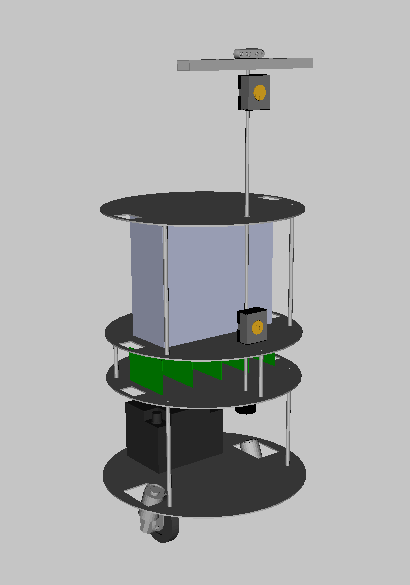
\includegraphics[width=0.3\textwidth]{robo_rviz.png}\\
    }
    % {\sourcecitation{Autor.}}
\end{figure}

Este robô já foi utilizado em trabalhos de conclusão de curso
anteriores, como em \textcite{petry_tcc} e \textcite{rahul_tcc}.
Porém, devido ao avanço do campo da robótica, ferramentas utilizadas
nesses trabalhos foram substituídas por novas versões, que
implementam técnicas modernas que serão abordadas ao longo do
trabalho. É o caso do ROS 2, sucessor do ROS 1, que é uma coleção de
bibliotecas e ferramentas para desenvolvimento de robôs, e do
\textit{Navigation 2}, um pacote para implementar navegação autônoma
em robôs móveis, que substituí o \textit{Navigation Stack} do ROS 1.

Neste trabalho, será dado seguimento ao desenvolvimento anterior no
Twil, com ajustes na odometria, além da adição de localização
utilizando uma câmera de profundidade e mapeamento do ambiente para
permitir a navegação autônoma em ambientes dinâmicos. Isto é feito
através da configuração de dois novos componentes, a câmera RGB-D
Intel RealSense D435 e uma unidade de medida inercial~(IMU). A imagem
da câmera é utilizada na odometria visual, na localização e no
mapeamento do ambiente, enquanto que as informações de orientação do
IMU são utilizadas para aprimorar a odometria do robô.

O mapa do ambiente tanto para o planejamento de trajetórias quanto
para a localização do robô. Como cada um destes sistemas tem
requisitos diferentes, foram criados dois mapas independentes.

\chapter{Revisão da Literatura}
\label{revisao}

Neste capítulo são apresentados os conceitos necessários para o
desenvolvimento do trabalho, como o Robot Operating System~(ROS) 2,
árvores de comportamento, mapeamento de ambientes e o
\textit{Navigation 2}.

\section{Robot Operating System 2 (ROS 2)}

O ROS 2 é a segunda geração do Robot Operating System, um
\textit{framework} para desenvolvimento de robôs. Ele foi
desenvolvido a partir do zero para atender as necessidades de robôs
modernos, com suporte para customização extensiva. O \textit{Data
    Distribution Service}~(DDS) é utilizado como o \textit{middleware},
que também é utilizado em sistemas de infraestrutura crítica, como
aplicações militares, aeroespaciais e financeiras. Este padrão
confere ao ROS ótima segurança e suporte para comunicação em tempo
real~\cite{ROS2Article}.

Um assunto relevante a este trabalho são os padrões de comunicação do
ROS 2. Existem três tipos de comunicação no ROS 2: \textit{topics},
\textit{services} e \textit{actions}. \textit{Topics} são canais de
comunicação unidirecionais, em que um nó, chamado de
\textit{publisher}, publica uma mensagem e outros nós, os
\textit{subscribers}, podem se inscrever no tópico publicado para
receber essa mensagem. \textit{Services} são um mecanismo do tipo
\textit{remote procedure call}~(RPC), em que um nó faz uma chamada a
outro nó que executa uma computação e retorna um resultado,
funcionando como um cliente e um servidor.

\textit{Actions}, são utilizados para tarefas de longa duração, com possibilidade de
cancelamento prematuro.
O cliente começa a execução enviando uma requisição para o servidor,
que response periodicamente com o estado atual da tarefa.
No término, é enviado o resultado, podendo ser sucesso ou falha.
Um exemplo de uso é uma tarefa de navegação em que um \textit{action client}
envia uma requisição com um ponto de destino para um \textit{action server}
que responde com realimentação contínua da posição atual do robô e
com o resultado ao finalizar a tarefa.
Eles também são apropriados para utilização em árvores de comportamento.

\section{Estimativa de posição de um robô móvel}

A terminologia e convenção dos sistemas de coordenadas de um robô
móvel utilizado neste trabalho é definido pela norma REP
105~\cite{rep_105}. Esta especificação define quatro sistemas de
coordenadas: \texttt{earth}, \texttt{map}, \texttt{odom} e
\texttt{base\_link}. Logo, a posição da base do robô, chamada de
\texttt{base\_link}, se da em relação a estes sistemas de
coordenadas.

O sistema de coordenadas chamado de \texttt{earth} é utilizado em
casos onde são utilizados múltiplos mapas, permitindo a interação
entre robôs de mapas diferentes. Neste trabalho, o foco é em um único
robô em um único mapa, portanto, este sistema de coordenadas não é
utilizado.

Assim, a posição do robô móvel será definida através das
transformadas entre os sistemas de coordenadas \texttt{map},
\texttt{odom} e \texttt{base\_link}. A transformada entre
\texttt{map} e \texttt{odom} será dada pelo sistema de localização,
enquanto que a transformada entre \texttt{odom} e \texttt{base\_link}
pelo sistema de odometria.

\todo[inline]{
    tenho que referenciar extensivamente isso nas duas seçoes seguintes

    https://www.ece.ufrgs.br/~fetter/ele00070/mobrob/estimation.pdf}

\subsection{Odometria}

A odometria publica a pose do robô em relação ao sistema de
coordenadas \texttt{odom}. Esta posição pode divergir ao longo do
tempo, sem limites, porém sua posição deve ser contínua. Devido a
essas características, ela é útil para referência local, mas deve ser
complementada com outros sistemas para referência global.

Essa odometria é geralmente obtida através de sensores incrementais,
como encoders nas rodas, que estimam a posição e orientação do robô
através da integração da velocidade das rodas. Devido a integração, a
estimativa de posição acumula erros ao longo do tempo.

Outros exemplos de fontes de odometria são Unidades de Medição
Inercial~(IMUs), que contém acelerômetros e giroscópios, e odometria
visual, que utilizam sensores óticos para estimar o movimento do
robô.

\todo[inline]{
    explicaçao de odometria visual usando ransac(que o rtabmap odom usa)
    que encontrei:

    doi: 10.1109/IMTIC.2018.8467263 }

\subsection{Localização}

O sistema de localização é responsável por publicar a transformada
entre os sistemas de coordenadas \texttt{map} e \texttt{odom}. A
posição do robô em relação ao \texttt{map} não deve divergir ao longo
do tempo significativamente, porém, esta coordenada não é continua e
a posição do robô pode mudar de forma abrupta em relação a ela. A
localização tem como intuito, portanto, corrigir os erros de posição
da odometria, publicando em uma frequência menor que a odometria um
ajuste da posição do robô.

Logo, devem ser utilizados sensores absolutos para localização, como
sensores baseados em visão computacional. Estes sensores utilizam
\textit{landmarks} obtidos através de um sensor ótico para estimar a
posição do robô em relação a eles. Estes sistemas não sofrem com
erros de acumulação, mas exigem processamento sofisticado,
ocasionando um longo tempo entre estimativas. Percebe-se que estes
sensores, portanto, são ideias para publicação da transformada entre
\texttt{map} e \texttt{odom}.

\section{Localização e Mapeamento Simultâneo (SLAM)}
\todo{acho que seria bom explicar melhor como funciona o slam, mencionando
    o loop closure}

Um campo de pesquisa importante na robótica móvel é o de localização
e mapeamento simultâneo~(SLAM). Introduzido em
~\textcite{slam_intro}, onde foi apresentado um método a partir de um
algoritmo baseado em um filtro de Kalman estendido, hoje aplicações
modernas utilizam técnicas baseadas em grafos, como detalhado em
\textcite{graph_slam}.

Entre pacotes que implementam o algoritmo baseado em grafos se
destacam o SLAM Toolbox e o Cartographer. Porém, o Cartographer foi
abandonado pelo Google e não é mais atualizado. O SLAM Toolbox, por
outro lado, foi escolhido como o pacote padrão de SLAM para o ROS 2,
e oferece diversas melhoras em relação a sistemas de SLAM anteriores,
como o GMapping, Karto, Hector e o próprio Cartographer. Estes
pacotes utilizam sensores em duas dimensões, sendo sensores baseados
em varrimento a laser os mais populares~\cite{SensorAndSLAM}.

Porém, com o avanço da tecnologia, sensores Red Green Blue -
Depth~(RGB-D) e câmeras estéreo estão se tornando mais acessíveis,
influenciando o desenvolvimento de sistemas de Visual~SLAM~(VSLAM).
Dentre sistemas de VSLAM, destacam-se o ORB-SLAM3, OpenVSLAM e
RTABMap, que possuem suporte a câmeras RGB-D e permitem localização
pura.

Em \textcite{VSLAM}, é feita uma comparação entre estes sistemas,
mostrando que o OpenVSLAM é a técnica mais adequada para maioria dos
casos. Dos pacotes citados neste artigo, apenas o RTABMap continua
sendo desenvolvido ativamente, com suporte as versões mais recentes
do ROS 2. Porém, novos sistemas de VSLAM promissores estão sendo
desenvolvidos, como o NVidia Isaac ROS VSLAM e o StellaROS, que é um
sucessor do OpenVSLAM.

\section{Fusão de dados de sensores}

Robôs modernos estão cada vez equipados com mais sensores,
ocasionando em mais uma fonte de dado para a mesma informação. Um
caso relevante neste trabalho, é a odometria do robô, que pode ser
estimada por diversos tipos de sensores, com diferentes
características. Ao invés de utilizar apenas um sensor para estimar a
odometria, os dados destes sensores, munidos da informação de
covariância do mesmo, podem ser fundidos obtendo uma estimativa mais
precisa. O filtro de Kalman, introduzido em \textcite{KalmanFilter},
é um estimador linear recursivo, comumente utilizado para aplicações
deste tipo.

Um exemplo de aplicação deste filtro para estimativa de posição no
ROS 2 é o pacote
\texttt{robot\_localization}~\cite{robot_localization_paper}. Este
pacote permite um número ilimitado de entrada de dados de sensores, e
tem suporte para diversos tipos de sensores, através da utilização de
diversos tipos de mensagens do ROS. Além disso, é possível configurar
os dados que serão utilizados de cada sensor, podendo ser excluídos
dados que não são relevantes ou confiáveis do resultado final.

\section{Mapas de custo}

Um mapa de custo é uma representação de ambiente composta por uma
grade de células que contém um valor, variando de desconhecido,
livre, ocupado ou custo inflado.

Em mapas de custo tradicionais, seus dados são armazenadas em mapas
monolíticos, para utilização em planejamento de trajetórias. Esta
implementação é utilizada com sucesso para caminhos curtos, mas pode
apresentar dificuldade em lidar com ambientes dinâmicos maiores.

Uma solução para este problema são mapas de custo com camadas, que
separam o processamento dos dados dos mapas de custos em camadas
semanticamente distintas~\cite{layered_costmaps}. Esta separação
permite a utilização de diferentes fontes de dados, permitindo, por
exemplo, adicionar dados de sensores para atualizar o mapa, sem
modificar o mapa original. Outras camadas podem ser configuradas para
evitar certas áreas, manter uma distância segura de obstáculos ou
seguir para seguir regras culturais, como manter a direita em
corredores. A Figura \ref{fig:mapa_camadas} mostra uma configuração
possível de camadas de mapas de custo.

\begin{figure}[h]
    {
        \centering
        \caption{Exemplo de configuração de camadas de um mapa de custo.}
        \label{fig:mapa_camadas}
        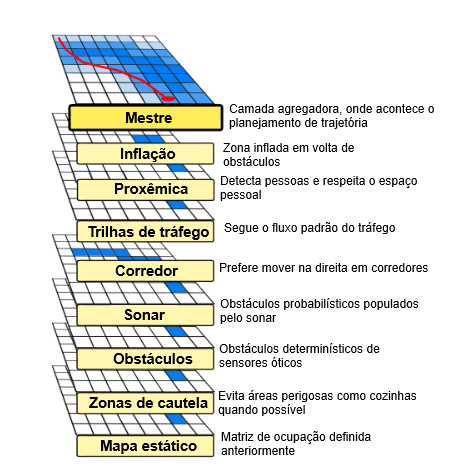
\includegraphics[width=0.5\textwidth]{mapa_camadas_trad.png}\\
    }
    {\sourcecitation{Adaptado de \textcite{layered_costmaps}.}}
\end{figure}

Três destas camadas são essenciais para mapear ambientes dinâmicos: a
camada estática, a camada de obstáculos e a camada de inflação. A
camada estática tem o mapa base, que deve ter apenas obstáculos
fixos, desta maneira, a trajetória planejada não será alterada em
razão de objetos inexistentes.

A camada de obstáculos é responsável por atualizar o mapa de custo
com obstáculos dinâmicos, através de dados de sensores óticos. Uma
opção desta camada é a camada \textit{voxel}, que utiliza uma
representação em três dimensões dos dados dos sensores, introduzida
em~\textcite{office_marathon}. Neste caso, é utilizado um espaço
tridimensional, composto por blocos chamados de \textit{voxels}, que
indicam se o bloco está ocupado ou livre. Cada coluna deste campo é
então projetada em um mapa bidimensional, com o valor dependendo da
presença de \textit{voxels} ocupados na mesma. Isto permite ao robô
detectar obstáculos em diferentes alturas, atualizando o mapa apenas
para obstáculos que podem colidir com o robô.

A camada de inflação utiliza os dados das camadas abaixo dela para
criar uma zona de segurança entre os obstáculos. Esta zona tem
valores intermediários entre os valores de obstáculo e livre, criando
trajetórias seguras mas que permitem que o robô passe próximo a
obstáculos, caso necessário.

\section{Navigation2}

O \textit{Navigation2}~(Nav2) é o sucessor do ROS \textit{navigation
    stack}, permitindo a realização de tarefas complexas em diversos
ambientes e classes de robôs cinemáticos. Baseando-se no legado do
\textit{navigation stack} do ROS 1, o Nav2 foi construído em cima do
ROS2, implementando técnicas mais modernas para ter um sistema
modular propício para ambientes dinâmicos com suporte a uma maior
variedade de sensores~\cite{Nav2}.

Uma árvore de comportamento é utilizada para orquestrar as tarefas de
navegação, ativando os servidores de controle, planejamento e
recuperação para navegação. Para executar nós de \textit{actions},
são normalmente utilizados \textit{Action servers} do ROS 2. Esta
árvore de comportamento pode ser configurada pelo usuário através de
um arquivo em XML, permitindo a descrição de comportamentos de
navegação únicos sem necessidade de programação.

Além disso, todos estes servidores utilizam o conceito de
\textit{Managed Nodes}, também conhecidos como \textit{Lifecycle
    Nodes}. Estes nós utilizam máquinas de estados para gerenciar seu
ciclo de vida, utilizando transições de estado desde sua criação a
destruição. No caso de falha ou desligamento, o nó vai do estado
ativo ao estado finalizado, seguindo a máquina de estados, permitindo
que o sistema seja interrompido de forma segura.

\todo{não acho que esse paragrafo ta bom}
Na arquitetura pode-se notar a utilização de dois mapas de custo, um
local e outro global. O mapa local, utilizado no servidor do
controlador, realiza o planejamento a curto prazo e prevenção de
colisão, enquanto o mapa global, aplicado no servidor de
planejamento, é usado principalmente para planejamento a longo prazo.

\chapter{Metodologia}
\label{desenvolvimento}

O sistema de navegação do Twil foi desenvolvido utilizando a versão
Humble do ROS 2, e com auxílio de ferramentas suportadas por esta
versão. Dentre as ferramentas utilizadas, destacam-se o Gazebo,
utilizado para simulação do robô, e o \textit{Navigation2}, que
fornece diversas ferramentas para implementar e orquestrar um sistema
de navegação autônoma.

Os variados componentes do robô, como os sensores utilizados neste
trabalho, foram implementados através de \textit{plugins} do Gazebo,
que comunicam o estado do robô durante a simulação através de tópicos
do ROS 2. A câmera RGB-D Intel RealSense D435, utilizada para o o
mapeamento do ambiente, foco deste trabalho, foi implementada desta
forma.

O \textit{Navigation2}, que tem sua arquitetura mostrada na Figura
\ref{fig:nav2_arc}, foi configurado para utilizar os componentes
disponíveis do robô Twil. O \textit{Nav2} é responsável pelo envio
comandos de velocidade para o robô, para que ele chegue ao destino
desejado de modo seguro, evitando colisões. Como pré-requisito, devem
ser fornecidos a este sistema a representação do ambiente, a posição
do robô neste ambiente, e um controlador para transformar os comandos
de velocidade em comandos para as rodas do robô.

\begin{figure}[h]
    {
        \centering
        \caption{Arquitetura do \textit{Navigation2}.}
        \label{fig:nav2_arc}
        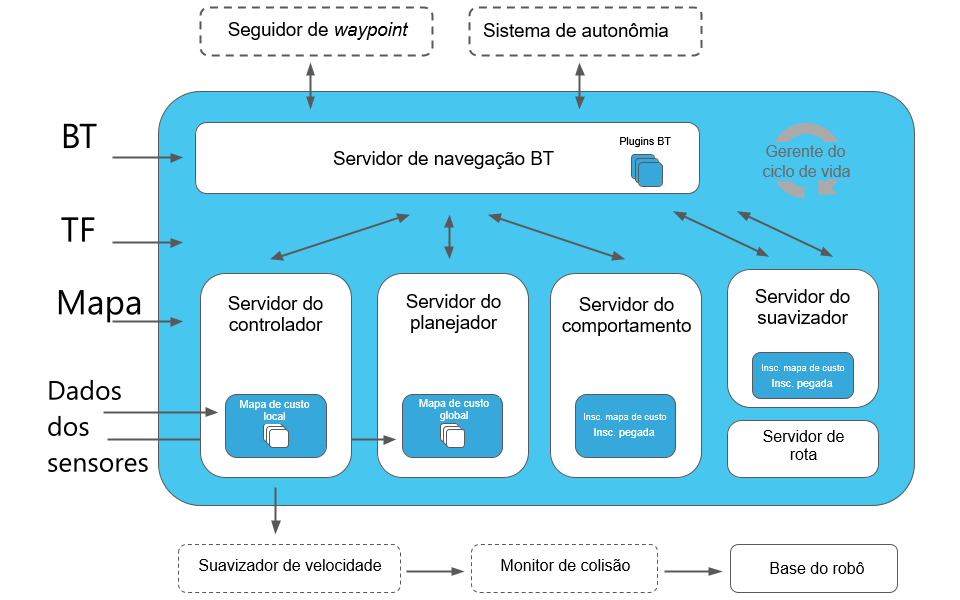
\includegraphics[width=0.9\textwidth]{nav2_architecture_trad.png}\\
    }
    {\sourcecitation{Adaptado de \textcite{nav2_site}.}} % colocar adaptado/traduzido?
\end{figure}

A representação do ambiente é feita através de um mapa de custo, e é
onde o servidor do planejador se baseia para construção de
trajetórias seguras do robô. A posição do robô é obtida através de
transformações entre os sistemas de coordenadas \texttt{map},
\texttt{odom} e \texttt{base\_link} do robô, conforme a especificação
REP 105~\cite{rep_105}. Esta posição é utilizada pelo servidor de
controlador para gerar comandos de velocidade para seguir a
trajetória planejada.

Antes do início deste trabalho, o Twil já estava configurada para
utilizar o \textit{Nav2}, porém sem utilizar dados da câmera e IMU.
Portanto, as trajetórias planejadas não eram atualizadas para evitar
obstáculos e não havia sistema de localização, ou seja, a
transformada entre \texttt{map} e \texttt{odom} era estática,
portanto não havia ajuste da odometria implementada.

Em razão disso, foi adicionada a câmera RGB-D Intel RealSense D435 e
um IMU ao robô, e o sistema de navegação foi aprimorado com a
utilização destes sensores nos sistemas de odometria, localização e
mapeamento.

Um diagrama simplificado da arquitetura do trabalho é mostrado na
Figura \ref{fig:arq_trabalho}. O desenvolvimento deste trabalho foi
focado nos componentes em vermelho, que realizam o mapeamento do
ambiente, e componentes em verde, que estimam a posição do robô. O
bloco em azul, que representa as outras ferramentas do \textit{Nav2},
e o controlador em amarelo, que transforma os comandos de velocidade
em comandos para as rodas do robô, já estavam configurados.

\begin{figure}[h]
    {
        \centering
        \caption{Arquitetura do simplificada do trabalho.}
        \label{fig:arq_trabalho}
        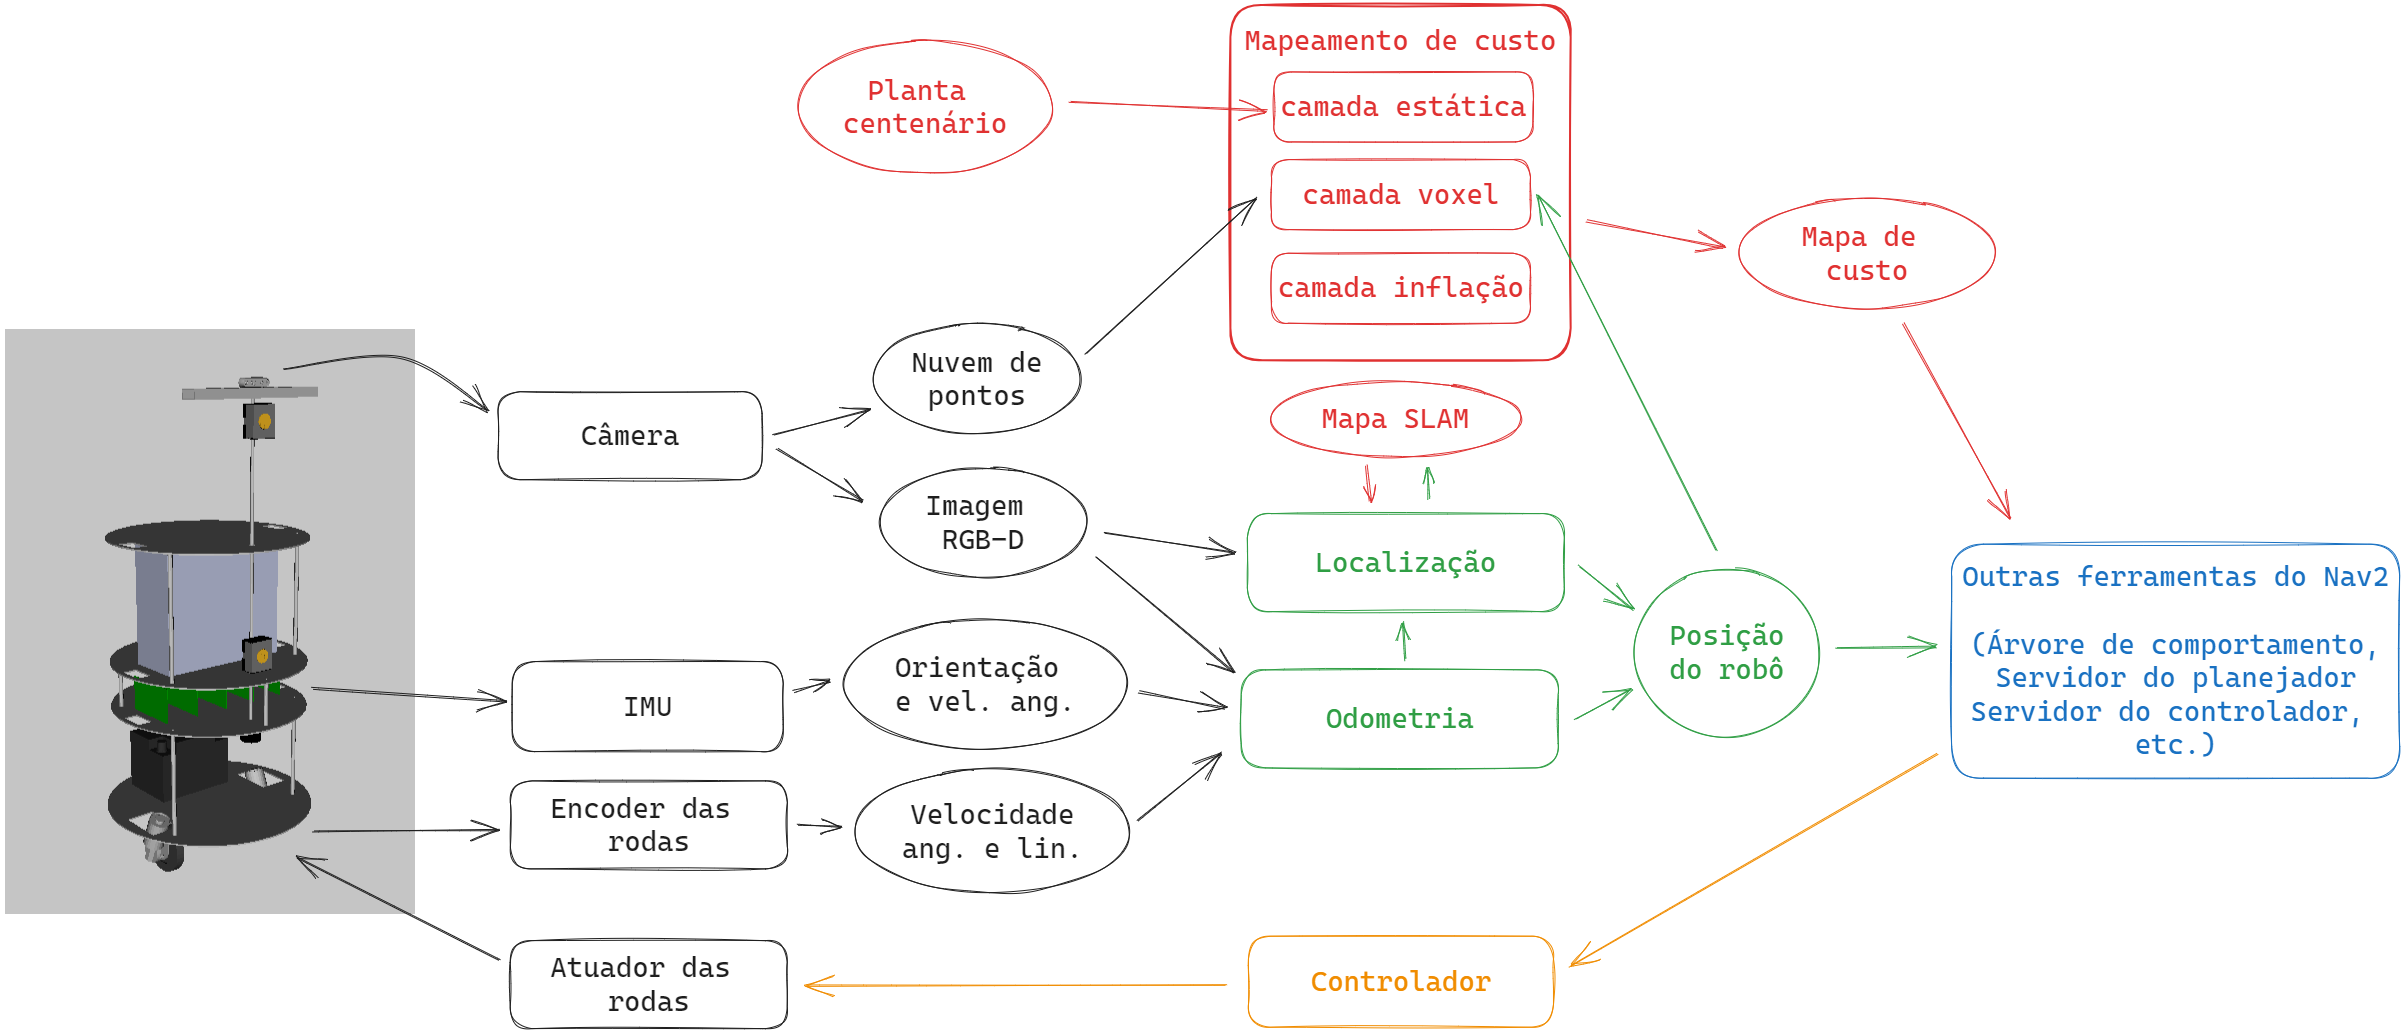
\includegraphics[width=0.98\textwidth]{arquitetura_simplificadav3.png}\\
    }
    % {\sourcecitation{Autor.}}
\end{figure}

Os componentes de mapeamento criam duas representações do ambiente.
Um mapa criado é o mapa de custo utilizado no planejamento de
trajetórias, onde foi adicionada uma camada para percepção de
obstáculos utilizando a câmera RGB-D. Além disso, foi realizada a
calibração da camada de inflação, para produzir caminhos mais
seguros. O segundo mapa é criado e utilizado pelos sistemas de
localização e mapeamento simultâneo~(SLAM), adicionados ao Twil.

Em verde, estão os componentes referentes a estimativa de posição do
robô, onde foram adicionados pacotes que realizam a odometria visual
e pacotes de SLAM. Também foi realizado ajustes na odometria das
rodas, através da fusão de dados com o sensor IMU. Ademais, para
realização de testes, foi mantida a opção de utilizar a transformada
estática entre \texttt{map} e \texttt{odom}, e foi adicionado um
sistema de odometria utilizando a posição exata do robô no Gazebo.

Nas seções seguintes, será apresentado o robô e o ambiente de testes
utilizado neste trabalho. Em seguida, será detalhado o
desenvolvimento dos sistemas necessários para a navegação autônoma do
robô neste ambiente. Finalmente, será descrita a coleta de dados para
a análise dos resultados, que é apresentada no próximo capítulo.

\section{Configuração do robô}

O modelo do robô está presente no pacote \texttt{twil\_description},
que contém os arquivos de descrição do robô no formato XACRO, que é
compilado para o formato URDF, utilizado pelo nodo
\texttt{robot\_state\_publisher}, que publica esta descrição em um
tópico. Este modelo é utilizado no rviz para visualização do robô,
como representado na Figura \ref{fig:robo_rviz}, e no Gazebo para
simulação. Para a simulação dos componentes físicos do robô, como
sensores e atuadores, são utilizados \textit{plugins} do Gazebo,
também presentes no arquivo de descrição.

Durante este trabalho, foram configurados dois novos componentes ao
robô, a câmera RGB-D Intel RealSense D435 e um IMU. A câmera foi
utilizada nos sistemas de odometria, localização e mapeamento,
enquanto o IMU foi usado como suplemento ao sistemas de odometria,
fornecendo dados de orientação do robô para fusão de dados.

Para utilização da câmera, é necessário o pacote
\texttt{realsense-ros}~\cite{realsense_ros}, que contém o modelo da
câmera. O \textit{plugin} do Gazebo \texttt{camera\_plugin}, é
responsável pela publicação dos dados da câmera simulada. São
utilizados cinco tópicos para publicar estes dados: dois tópicos são
utilizados para publicar as imagens não comprimidas, uma RGB e outra
de profundidade; dois tópicos com informações destas imagens; e um
tópico com a nuvem de pontos produzida pela câmera.

A adição do IMU foi feita utilizando o \textit{plugin}
\texttt{GazeboRosImuSensor}, que publica mensagens do tipo
\texttt{sensor\_msgs/Imu}. Estas mensagens contêm a orientação,
velocidade angular e aceleração linear do robô. Por si só, o IMU não
é confiável para estimar a posição do robô porque porque necessita
integrar a aceleração linear duas vezes para estimar a posição, que
pode introduzir erros significativos. Porém, os dados referentes a
orientação e velocidade angular podem ser fundidos com outras fontes
de odometria para complementar outras fontes de odometria. Para
representar fisicamente o IMU no robô, foi reutilizada a descrição de
uma placa de circuito impresso \textit{Eurocard}, já utilizada em
outros componentes do robô.

A conversão dos comandos de velocidade em movimento de rodas do robô
é feita pelo controlador, configurado no pacote
\texttt{twil\_bringup}. Diversos controladores estão configurados e
disponível para uso com o Twil, porém o controlador
\textit{twist\_mrac\_controller}, do pacote
\texttt{linearizing\_controllers} foi o escolhido e configurado para
ser usado com o \textit{Nav2} em trabalhos anteriores.

\section{Ambiente de simulação}

O sistema será simulado em uma simulação do prédio Centenário da
Escola de Engenharia da UFRGS, utilizando o Gazebo. No pacote
\texttt{ufrgs\_map} está incluído uma representação em formato PGM da
planta do prédio, mostrada na Figura \ref{fig:planta_centenario},
desenvolvida em \textcite{petry_tcc} Além da imagem da planta, também
está presente um arquivo de configuração em formato YAML, que contém
a resolução, origem do mapa. Este arquivo de também contém parâmetros
para utilização como mapa de custo, indicando a faixa de valores para
considerar uma célula como livre ou ocupada.

\begin{figure}[h]
    {
        \centering
        \caption{Planta do 1º andar do prédio Centenário da EE-UFRGS.}
        \label{fig:planta_centenario}
        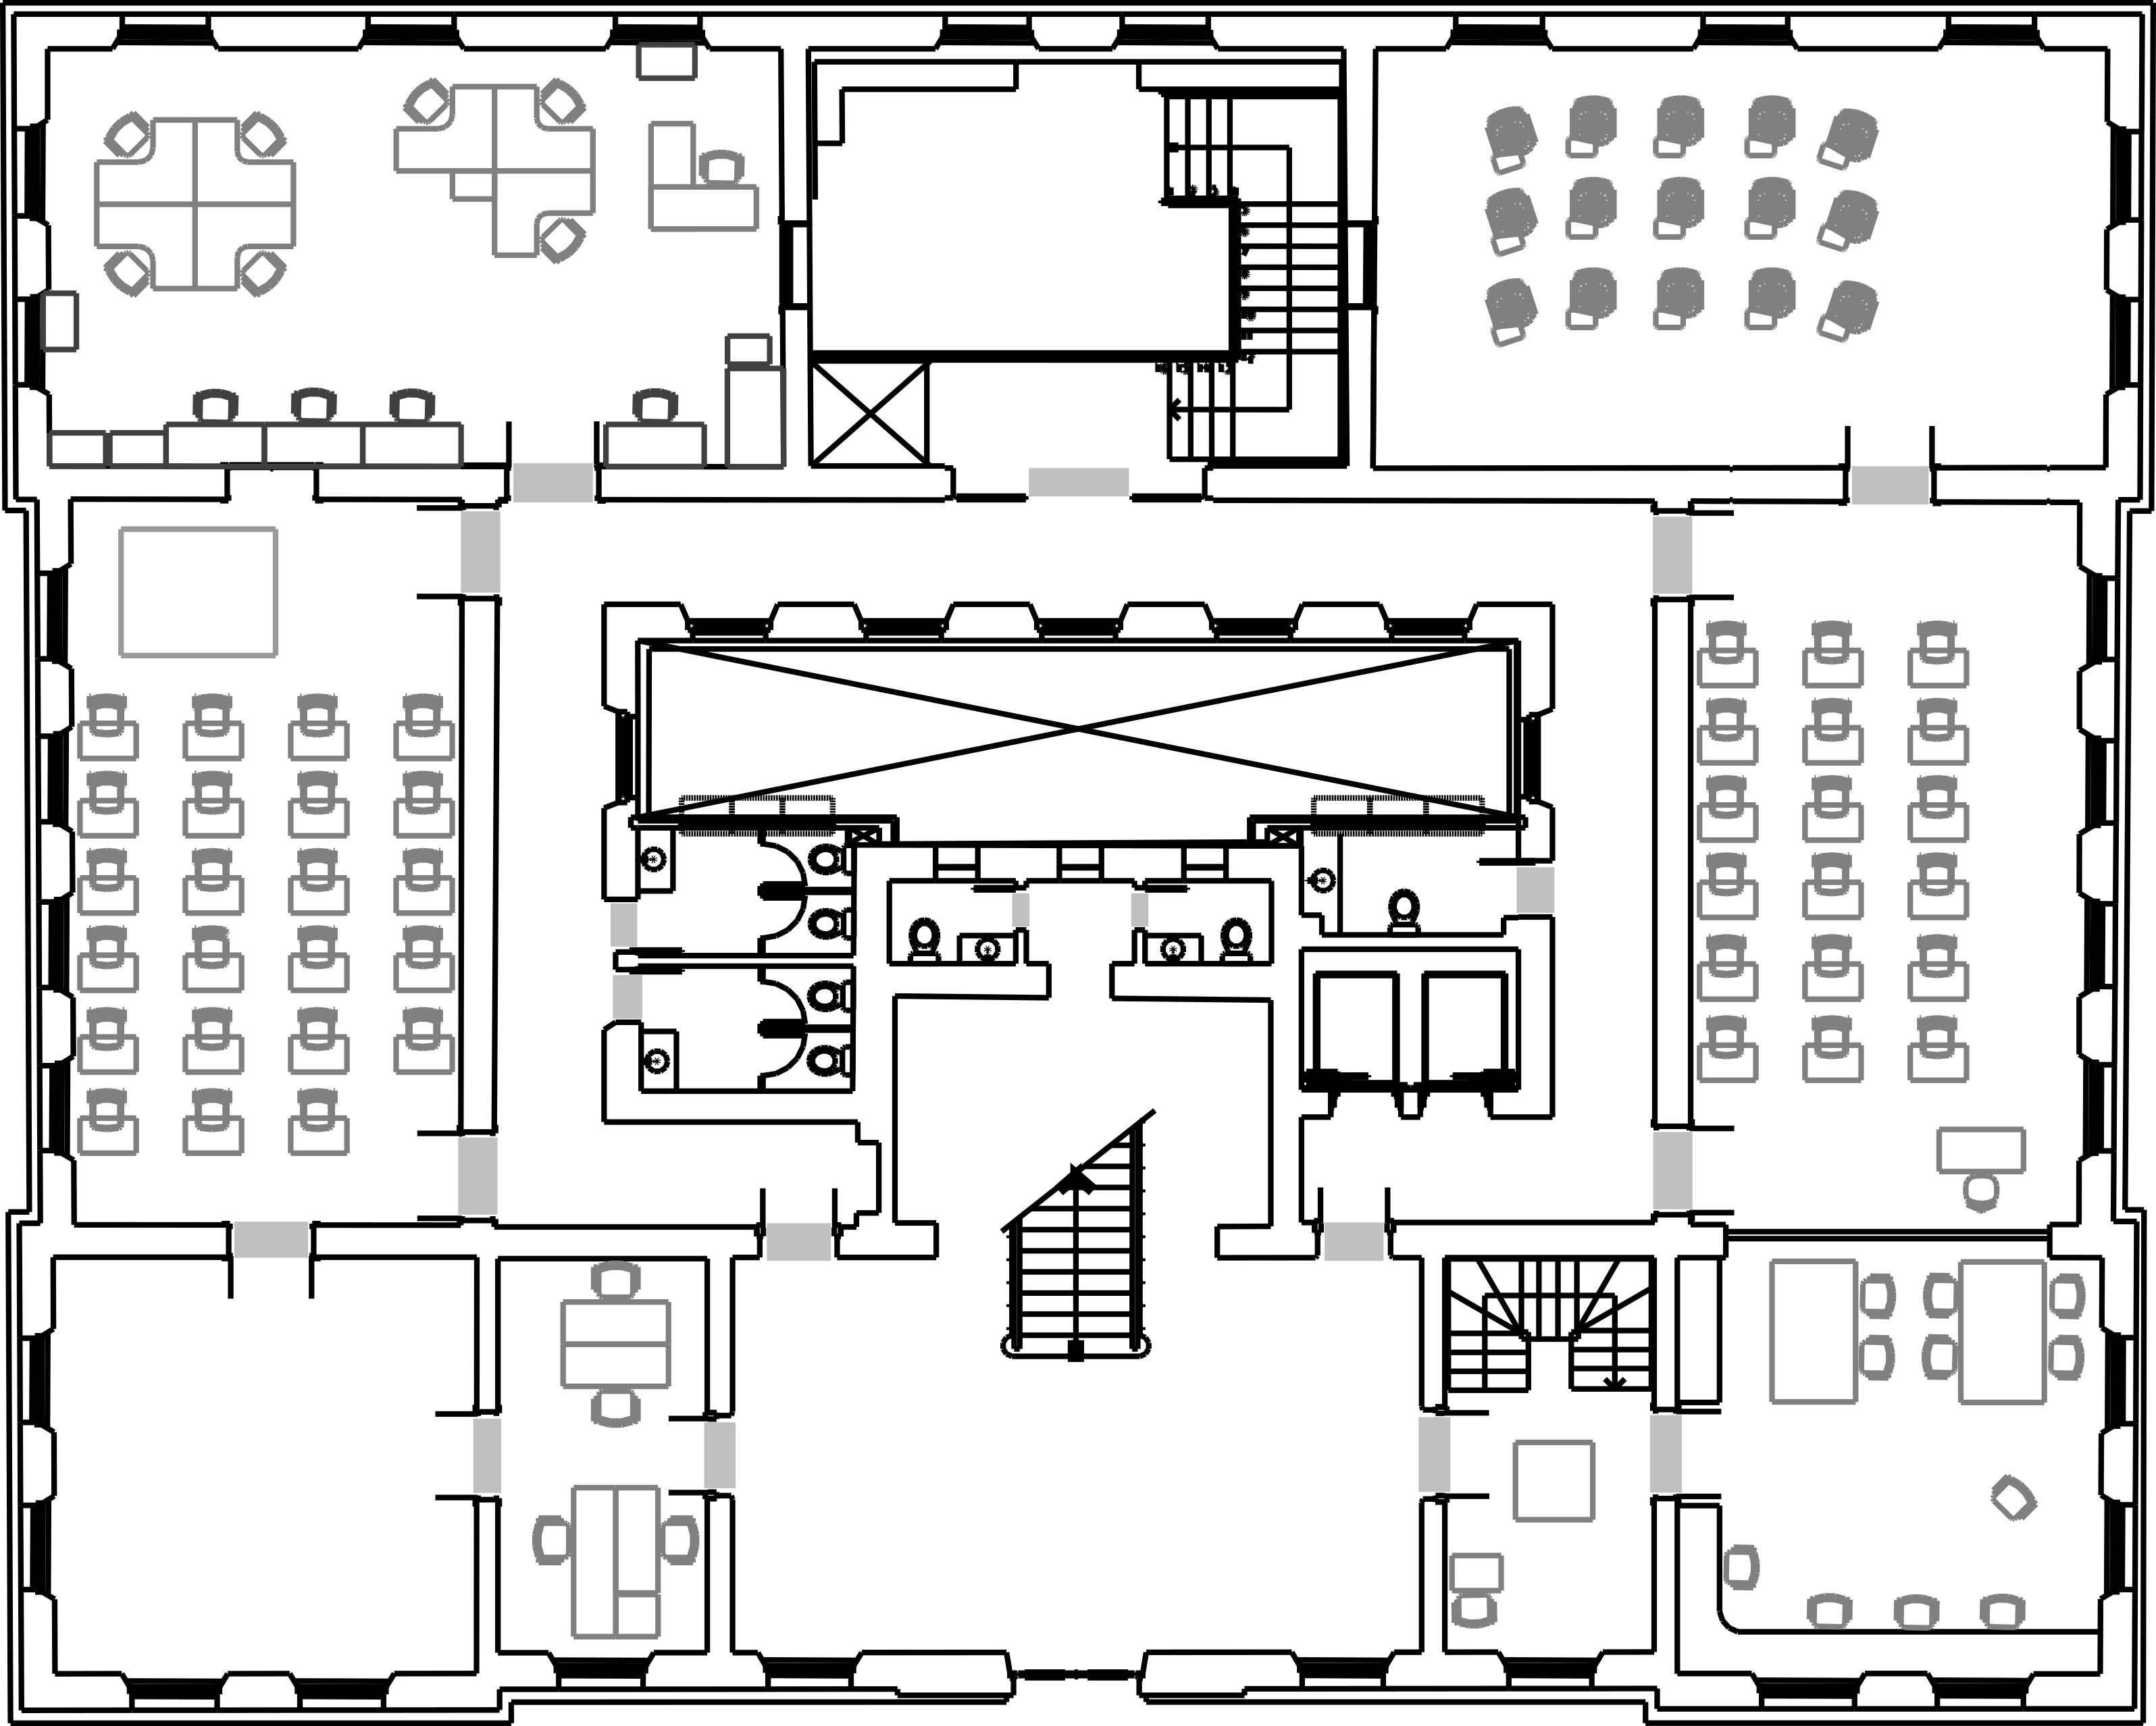
\includegraphics[width=0.7\textwidth]{centenario_floor_plan.png}\\
    }
    {\sourcecitation{\textcite{petry_tcc}.}}
\end{figure}

O pacote \texttt{ufrgs\_gazebo} contém arquivos de mundos do Gazebo
para simulação. Este pacote, porém, estava desatualizado e não
continha uma representação completa do prédio Centenário. Utilizando
o \textit{Building Editor} do Gazebo, foi criado um modelo
simplificado do prédio em 3D, com base na sua planta, mostrado na
Figura \ref{fig:gazebo_centenario}.

\begin{figure}[h]
    {
        \centering
        \caption{Ambiente Gazebo com modelo do prédio Centenário da EE-UFRGS.}
        \label{fig:gazebo_centenario}
        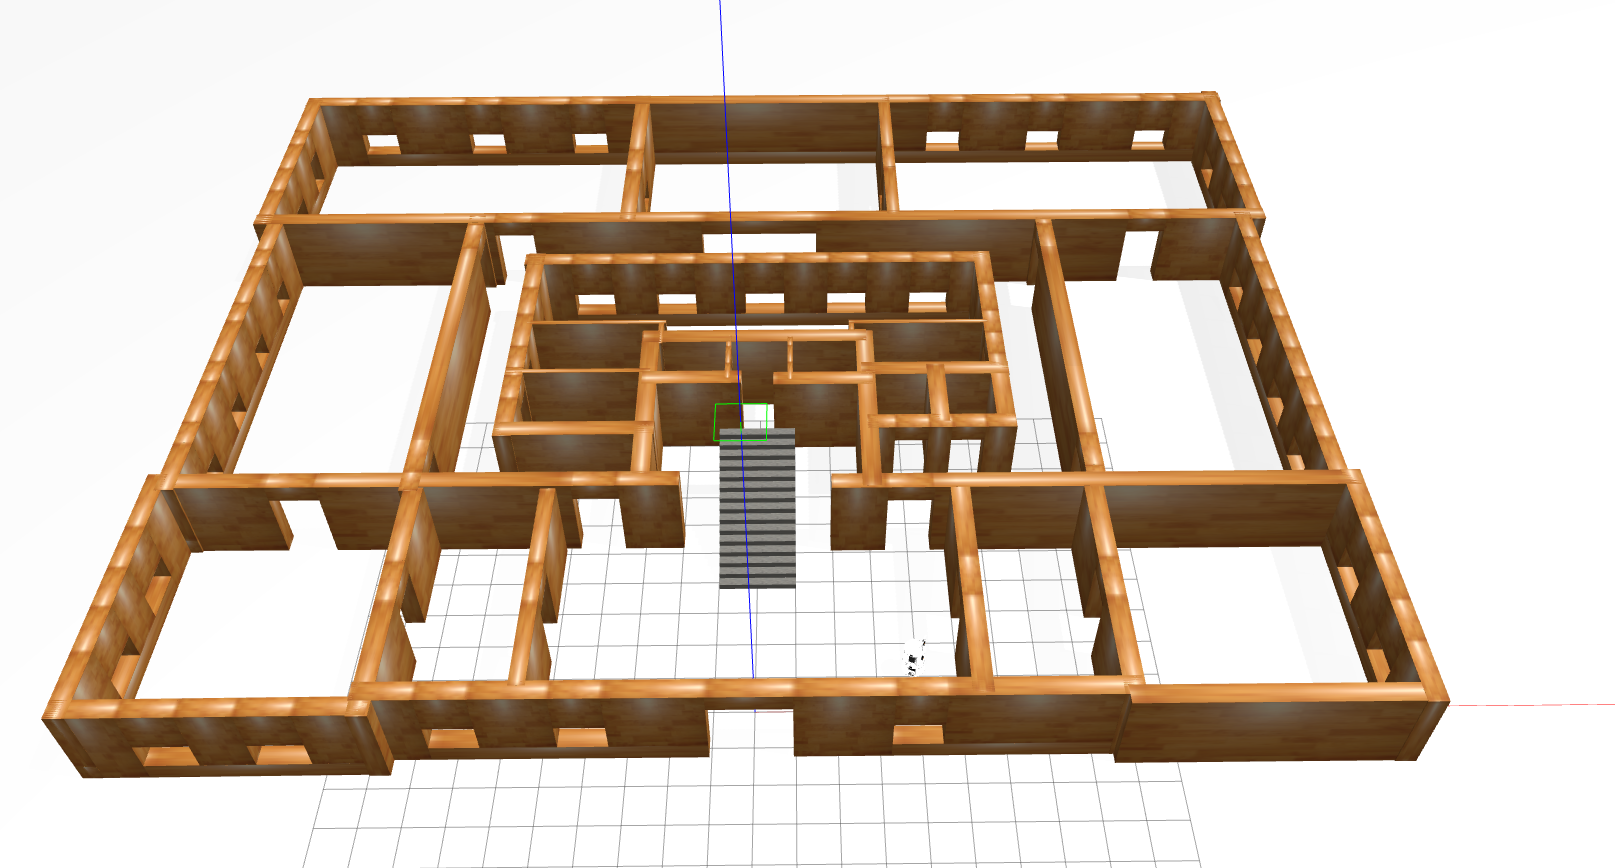
\includegraphics[width=0.95\textwidth]{gazebo.png}\\
    }
    % {\sourcecitation{Autor.}}
\end{figure}

Não foram adicionados os obstáculos em cinza claro da planta da
Figura \ref{fig:planta_centenario}, que não são obstáculos fixos.
Para teste com obstáculos dinâmicos ou temporário são adicionados
novos objetos a este mundo durante a execução da simulação no Gazebo.

\section{Estimativa de posição do robô}

A estimativa de posição é feita utilizando o sistemas de coordenadas
definido pela norma REP 105~\cite{rep_105}, que define quatro
sistemas de coordenadas: \texttt{earth}, \texttt{map}, \texttt{odom}
e \texttt{base\_link}. Como só é utilizado um mapa, o sistema de
coordenadas \texttt{earth} não é utilizado. Todas transformadas entre
estes sistemas de coordenadas são publicadas no tópico \texttt{tf},
por padrão do ROS 2. Estas transformadas são publicados por dois
sistemas, o de odometria e de localização.

\subsection{Odometria}
\label{met:odometria}

O sistema de odometria é responsável pela publicação da transformada
entre o sistema de coordenadas \texttt{odom} e \texttt{base\_link}. A
posição do robô em relação ao \texttt{odom} deve ser contínua, porém
pode divergir gradualmente. Por esta razão, são geralmente utilizados
sensores incrementais na odometria, que estimam a posição e
orientação do robô por integração e, portanto, são suscetíveis a
erros de acumulação. \todo{eu basicamente repeti o que escrevi na
    revisao da literatura aqui, talvez seja uma boa ajustar isso}

Neste trabalho, serão utilizados e comparados três sistemas de
odometria, que além da transformada, também publicam mensagens do
tipo \texttt{nav\_msgs/Odometry} no tópico \texttt{/odom}. Antes
deste trabalho, a odometria era publicada apenas pelo controlador,
através do pacote \texttt{twist\_mrac\_controller}, utilizando dados
do encoder nas rodas para estimar a posição do robô. O cálculo da
posição é feito pelo pacote \texttt{arc\_odometry}, que utiliza o
modelo cinemático de um robô móvel de acionamento diferencial para
estimar a posição e orientação do robô a partir das posições de junta
das rodas. Para aprimorar a qualidade desta odometria, foi adicionado
o pacote \texttt{robot\_localization}, que realiza a fusão de de
dados da odometria das rodas com os dados do IMU.

\todo[inline]{
    reescrever e explicar melhor a parte da utilizacao da velocidade
}
A fusão é realizada através de um filtro de Kalman estendido, onde
devem ser escolhidos quais dados dos sensores devem ser considerados.
Apesar da recomendação de configuração dos criadores do pacote, onde
é sugerido utilizar apenas dados de velocidade e não de posição
\cite{robot_localization_guide}, para os dados calculados pelo
\texttt{arc\_odometry}, decidiu-se utilizar tanto a posição quanto a
velocidade na fusão de dados. Isso foi feito porque a velocidade
calculada pelo \texttt{arc\_odometry} é calculada em referência ao
sistema de coordenadas global, neste caso, o \texttt{odom}, enquanto
que o \texttt{robot\_localization} espera que a velocidade seja em
referência a base do robô. Portanto, a posição calculada pelo
\texttt{robot\_localization} com a velocidade publicado pelo
\texttt{arc\_odometry} não é correta.

Porém, utilizando os dados de posição da odometria de rodas, não é
usado a velocidade para calcular a posição. Desta forma, a posição
publicada pelo \texttt{robot\_localization} é a mesma que a publicada
pelo \texttt{arc\_odometry}, já que esta é a única fonte de dados de
posição. Porém, a orientação e velocidade angular da odometria das
rodas são fundidas com os dados do IMU, melhorando a precisão destes
campos na mensagem publicada.

\todo{ eu traduzi
    "features" como caracteristicas, mas talvez seja um termo especifico
    de visao computacional }

Como alternativa a este sistema, foi implementado um sistema de
odometria visual, publicado pelo executável \texttt{rgbd\_odometry}
do pacote \texttt{rtabmap\_odom}, que utiliza imagens da câmera RGB-D
com auxílio do sensor IMU para estimava da posição. Utilizando
características das imagens RGB, com a informação de profundidade da
imagem de profundidade, é utilizado um método \textit{Random Sample
    Consensus} (RANSAC), para comparar imagens consecutivas e estimar a
velocidade do robô\cite{rtabmap_odom}.

É possível, fundir os dados destes dois sistemas de odometria,
porém, optou-se por mantê-los separados para facilitar a comparação
do desempenho entre eles.

Finalmente, para realização de testes, foi implementado um sistema de
odometria com a posição real do robô no Gazebo. Utilizando o
\textit{plugin} P3D, é publicada uma mensagem do tipo
\texttt{nav\_msgs/Odometry} com a posição do robô em relação ao
sistema de coordenadas \texttt{odom} a um tópico auxiliar. Quando
está sendo utilizado este sistema de odometria, o que é publicado
neste tópico é retransmitido para o tópico \texttt{/odom} e o pacote
\texttt{odom\_to\_tf\_ros2} publica a transformada entre
\texttt{odom} e \texttt{base\_link} com base no dado de posição da
mensagem publicada.

Os sistemas de odometria utilizados, estão resumidos na Tabela
\ref{tab:odometria}, onde é indicado o pacote, a fonte de dados e o
tipo de mensagem recebido por cada um.

\begin{table}[h]
    \begin{center}
        \caption{Sistemas de odometria}
        \label{tab:odometria}
        \begin{tabular}{c|c|c}
            Pacote utilizado                              & Fonte de dados          & Tipo de mensagem recebida                       \\
            \hline
            \multirow{2}{*}{\texttt{robot\_localization}} & Encoder das rodas       & \texttt{nav\_msgs/Odometry}                     \\
                                                          & IMU                     & \texttt{sensor\_msgs/Imu}                       \\
            \hline
            \multirow{3}{*}{\texttt{rtabmap\_odom}}       & \multirow{2}{*}{Câmera} & \texttt{sensor\_msgs/CameraInfo}                \\
                                                          &                         & \texttt{sensor\_msgs/Image}(RGB e profundidade) \\
                                                          & IMU                     & \texttt{sensor\_msgs/Imu}                       \\
            \hline
            \texttt{odom\_to\_tf\_ros2}                   & Posição no Gazebo       & \texttt{nav\_msgs/Odometry}                     \\
        \end{tabular}
    \end{center}
    % {\sourcecitation{Autor}}
\end{table}
\todo[inline]{
    a camera no rgbd odom usa dois topicos do do tipo image,
    por isso que coloquei "(rgb e profundidade)",
    mas achei que ficou estranho

    talvez faça sentido colocar o tipo de mensagem image duas vezes e
    colocar rgb numa e profundidade na outra }

\subsection{Localização}
\label{met:localizacao}

O sistema de localização, por outro lado, publica a transformada
entre o sistema de coordenadas \texttt{map} e \texttt{odom}. Este
transformada não deve acumular erros, porém não precisa ser contínua.
Por esta razão, são utilizados principalmente sensores absolutos, que
podem ter alta complexidade de processamento, já que não precisam ser
atualizados em alta frequência, como a odometria.

Estes sistemas, portanto, servem para ajustar os erros de odometria.
Anteriormente, não era utilizado nenhum sensor para localização do
robô, e a transformada entre \texttt{map} e \texttt{odom} era
estática, causando divergência na estimativa de posição durante a
navegação. Este sistema foi mantido para testes, porém foram
implementados dois sistemas de localização baseados em localização e
mapeamento simultâneos(SLAM), utilizando a câmera RGB-D Intel
RealSense D435, para melhorar a estimativa de posição do robô
publicada pela odometria.

Uma alternativa à sistemas SLAM é o \texttt{nav2\_amcl}, que utiliza
localização por Monte Carlo com um mapa construída previamente, que
poderia ser a planta do prédio, para estimar a posição do robô.
Porém, opção foi descartada, pois o objetivo é a utilização do robô
em ambiente dinâmicos ou pouco conhecidos, onde um mapa estático não
seria adequado. Além disso, este pacote só é compatível com
representações bidimensionais do ambiente, que causaria problemas na
detecção de objetos tridimensionais como as escadas, agravando as
diferenças já existem entre o ambiente do Gazebo e a planta.

Os dois sistemas de SLAM utilizados foram o \texttt{slam\_toolbox} e
o \texttt{rtabmap\_slam}, resumidos na Tabela \ref{tab:localizacao}.

\begin{table}[h]
    \begin{center}
        \caption{Sistemas de localização}
        \label{tab:localizacao}
        \begin{tabular}{c|c|c}
            Pacote utilizado                        & Fonte de dados          & Tipo de mensagem recebida                       \\
            \hline
            \texttt{slam\_toolbox}                  & Câmera                  & \texttt{sensor\_msgs/LaserScan}                 \\
            \hline
            \multirow{2}{*}{\texttt{rtabmap\_slam}} & \multirow{2}{*}{Câmera} & \texttt{sensor\_msgs/CameraInfo}                \\
                                                    &                         & \texttt{sensor\_msgs/Image}(RGB e profundidade) \\
        \end{tabular}
    \end{center}
\end{table}

O \textit{slam\_toolbox}, realiza o SLAM em 2D, e foi criado para
utilizar sensores a laser. Portanto, são esperadas mensagens do tipo
\texttt{sensor\_msgs/LaserScan} para percepção do ambiente neste
sistema. Como a câmera RGB-D não publica mensagens desse tipo, o
pacote \texttt{depthimage\_to\_laserscan} foi usado para converter a
imagem de profundidade da câmera na mensagem esperada, em forma de um
feixe de luz em duas dimensões localizado na altura da câmera. O
\textit{rtabmap}, por outro lado, realiza o SLAM em 3D, e utiliza
todos os tópicos publicados pela câmera RGB-D, e não necessita de
conversão de mensagens.

Ambos sistemas publicam a transformada entre \texttt{map} e
\texttt{odom}, além da posição global do robô no tópico
\texttt{/pose}, em mensagens do tipo
\texttt{geometry\_msgs/PoseWithCovarianceStamped}, que são utilizadas
para comparação com a posição real e a estimada pela odometria.

Apesar de realizar o mapeamento do ambiente em tempo-real, estes
sistemas podem ser iniciados com informações de uma sessão prévia de
mapeamento, que pode aumentar a precisão da localização, caso o mapa
seja mais fiel que o construído. Porém, nos testes realizados, a
sessão de SLAM foi iniciada do zero, para simular um ambiente
desconhecido.

\section{Mapeamento}

O mapeamento é um aspecto essencial para a navegação autônoma. Ele é
utilizado tanto no planejador de trajetórias, para perceber e evitar
obstáculos dinâmicos, quanto no sistema de localização do robô, para
estimar a posição do robô no ambiente.
% O mesmo mapa poderia ser
% utilizado para ambos sistemas, porém, devido a diferentes
% necessidades de cada sistema, optou-se criar dois mapas do ambiente,
% o mapa de custo, para planejamento de trajetórias, e o mapa SLAM,
% utiliza para localização do robô.

Apesar do sistema de SLAM fornecer um mapa do ambiente, este mapa não
será utilizado no mapa de custo. Como este mapa não está completo
desde o início, não é possível planejar trajetórias para ambientes
não visitados previamente. Além disso, é preferível que o mapa da
camada estática tenha apenas obstáculos fixos, como paredes e
escadas, e utilizar a camada de obstáculos para obstáculos dinâmicos.
Esta separação permite que o mapa estática seja utilizado em diversas
sessões, porém com uma camada de obstáculos nova a cada sessão. Além
disso, a camada de obstáculos pode ser configurada de forma
independente que o SLAM, podendo utilizar outros sensores ou
considerar uma altura de obstáculos diferente.

Portanto, haverão duas representações do ambiente, uma criada pelo
SLAM, que é utilizada apenas para localização, e outra criada
utilizando os \textit{plugins} do mapa de custo do Nav2, que é
utilizada para planejamento de trajetória.

\subsection{Mapeamento de custo}

O mapa de custo utilizado é composto por três camadas: a camada
estática, que possui uma representação simples do ambiente,
preferencialmente sem obstáculos temporários; a camada de obstáculos
ou \textit{voxel}, onde são utilizados dados dos sensores óticos para
atualizar o mapa com obstáculos percebidos; e a camada de inflação,
que cria um campo de custo ao redor dos obstáculos.

A planta do prédio Centenário, representada na Figura
\ref{fig:planta_centenario}, foi utilizada como mapa estático. O mapa
foi configurado para considerar apenas as cédulas em preto escuro
como ocupados, que equivalem a obstáculos fixos, como paredes e a
escada. As cédulas em cinza claro são consideradas livres, que
representam a posição provável de objetos móveis, como cadeiras e
mesas.

A camada de obstáculos utiliza os dados da camera RGB-D para
atualizar o mapa. Existem dois \textit{plugins} que podem ser
utilizados para este fim, o \texttt{obstacle\_layer} e o
\texttt{voxel\_layer}. Ambos podem utilizar mensagens do tipo
\texttt{PointCloud2}, que são publicadas pela câmera RGB-D, porém
utilizam técnicas diferentes para atualizar o mapa. \todo{nao achei
    traducao para ray casting} O \texttt{obstacle\_layer} utiliza
\textit{ray casting} em 2D para determinar a posição dos obstáculos.
O \texttt{voxel\_layer}, por outro lado, cria um gride
tri-dimensional, divido em blocos chamados de \textit{voxels}, que
podem estar ocupados ou livres.

Apesar do mapa de custo ser em 2D, a simulação e o mundo real podem
ter obstáculos de diferentes alturas, como mesas e cadeiras.
Portanto, é necessária a percepção em 3D do ambiente para evitar
colisões com estes obstáculos. Logo, foi utilizado o
\texttt{voxel\_layer} para atualizar o mapa de custo.

Para a configuração do \texttt{voxel\_layer}, é necessário definir a
resolução e o número de \textit{voxels} no eixo Z utilizados. A
câmera RGB-D Intel RealSense D435 do Twil está localizada a uma
altura de aproximadamente 1,37 metros do chão, que é a altura mínima
do gride de \textit{voxels}. O número máximo de \textit{voxels}
permitido pelo \textit{plugin} é 16. Tendo em vista estes dados, foi
definido um gride de \textit{voxels} com 15 \textit{voxels} de
resolução 0,1 metro, criando um gride de 1,5 metro de altura.
Portanto, serão captados obstáculos dentro deste campo, porém
obstáculos com altura superior a 1,5 metro não serão detectados. Isso
é importante para evitar a detecção de obstáculos que não são
relevantes para a navegação como, no caso do ambiente de simulação
utilizado, a moldura das portas.

A última camada, \texttt{inflation\_layer}, cria uma zona de
segurança ao redor dos objetos captados nas outras camadas, para
garantir uma distância segura ao planejar a trajetória. Em
\textcite{ros_tuning_guide}, recomenda-se que a camada de inflação
cubra um raio grande em volta de obstáculos com uma curva de
decaimento de inclinação baixa, criando um campo em grande parte do
mapa de custo. Desta forma, são criadas trajetórias que passam no
meio de obstáculos, mantendo a maior distância possível entre o robô
e possíveis colisões.

\todo[inline]{
    daria pra fazer uma tabela igual ao dos sistemas de odometria
    e localizacao, só que cada linha é uma camada do mapa de custo
}

\subsection{Mapeamento SLAM}

O mapeamento realizado pelo sistemas SLAM é utilizado apenas para a
localização do robô pelo mesmo pacote que o criou. Foram criados dois
mapas, um por cada pacote de localização implementado,
\texttt{slam\_toolbox} e \texttt{rtabmap\_slam}, descritos na Seção
\ref{met:localizacao}.

Devido aos dados dos sensores utilizados o \texttt{slam\_toolbox} é
capaz de criar mapas apenas em duas dimensões. Porém, o
\texttt{rtabmap\_slam} pode criar mapas em duas ou três dimensões.
Como o robô Twil não é capaz de se movimentar em três dimensões,
neste trabalho só serão comparados os mapas em 2D criados por ambos
pacotes.

\todo[inline]{
    poderia escrever mais nessa seção talvez

    acho que podia falar um pouco sobre o loop closure aqui e porque nao
    testei em outro lugar(bag ficava muito grande porque o mapa é muito
    grande) }

\section{Testes e coleta de dados}
\label{met:testes}

Devido a independência entre o mapeamento de custos e os demais
sistemas desenvolvidos neste trabalho, foram realizados dois tipos de
de testes diferentes. Para testar o mapeamento de custo, foram
executadas criadas trajetórias com e sem obstáculos para testar a
performance das camadas de obstáculos e inflação. Para testar os
sistemas de odometria, localização e mapeamento SLAM, foram
utilizados arquivos de gravação de tópicos do ROS 2, chamados de
sacolas, ou em inglês, \textit{bags}.

Estas sacolas permite a execução de diversas simulações usando os
mesmos dados de entrada. Outro benefício foi o alivio na exigência de
processamento do computador utilizado, já que foi realizar a
simulação no Gazebo e executar os nodos de localização separadamente.

Para a gravação das sacolas, foi criado um programa em \textit{bash}
que contêm todos os tópicos necessários para a execução dos sistemas
de odometria e localização, além de tópicos auxiliares para
comparação com a posição real do robô e visualização no rviz, como o
tópico \texttt{/ground\_truth}, que contém a posição real do robô,
publicado pelo \textit{plugin} P3D do Gazebo. Este tópico difere do
tópico criado por este \textit{plugin} utilizado no sistema odometria
porque a posição deste é publicada em relação ao sistema de
coordenadas \texttt{map} e não \texttt{odom}.

Os tópicos necessários para a execução dos sistemas de odometria
estão nas Tabelas \ref{tab:odometria} e \ref{tab:localizacao},
descritos anteriormente. Porém, além destes que são inscritos
explicitamente na configuração do pacote, os sistemas de odometria e
localização que utilizam a câmera RGB-D também utilizam o tópico
\texttt{/tf}, que contém a árvore de transformadas da base do robô
até a câmera. Esta transformação é necessária para a utilização dos
dados da câmera. Portanto, esta informação deve estar presente
durante a execução dos testes.

Uma solução para disponibilizar esta transformada seria gravar o
tópico \texttt{/tf} durante a execução da simulação. Porém, isto não
é possível, porque este tópico já possui as transformadas entre
\texttt{map}, \texttt{odom} e \texttt{base\_link}, o que causaria
conflitos com as transformadas publicadas pelos sistemas de odometria
e localização sendo testados. Logo, durante a execução dos testes,
devem ser publicadas as mesmas transformadas que foram publicadas
durante a gravação da sacola.

A transformação das juntas do robô são publicadas pelo
\texttt{robot\_state\_publisher}. Existem dois tipos de juntas entre
a base do robô e a câmera: estáticas, que tem sua informação definida
no arquivo de descrição do robô, e dinâmicas, que são publicadas pelo
Gazebo, através das configurações definidas no
\texttt{twil\_bringup}, no tópico \texttt{joint\_states}. O
executável \texttt{robot\_state\_publisher} utiliza este tópico e o
arquivo de descrição para publicar as transformadas entre os
componentes do robô no tópico \texttt{/tf}. Portanto, para evitar a
execução do Gazebo, este tópico foi gravado na sacola, e foi
executado o \texttt{robot\_state\_publisher} com o arquivo de
descrição do robô, obtendo assim, o mesmo estado do robô durante a
execução da simulação utilizada para a gravação da sacola.

Para facilitar a execução deste publicador de transformadas do robô e
dos sistemas de odometria e localização, foi criado um arquivo de
inicialização com os nodos necessários para realizar os testes com as
informações da sacola.

Os resultados dos testes foram analisados utilizando o programa
\textit{Plotjuggler}~\cite{plotjuggler}, que permite criar gráficos
de tópicos do ROS em tempo real ou a partir de uma sacola. Optou-se
por criar outro programa em \textit{bash} para gravar os tópicos do
testes para criação dos gráficos no \textit{Plotjuggler}. Desta
forma, os dados dos testes ficam gravados e podem ser analisados
posteriormente.

Os gráficos foram construídos utilizando os dados de posição x e y
das mensagens do tipo \texttt{nav\_msgs/Odometry} publicadas pelos
sistemas de odometria e pelo Gazebo com a posição real do robô. Para
o sistemas de localização, foram utilizados os dados de posição x, y
das mensagens do tipo
\texttt{geometry\_msgs/PoseWithCovarianceStamped}, que são referentes
a posição global do robô calculada por estes pacotes, ou seja, a
transformada entre \texttt{map}, \texttt{odom} e \texttt{base\_link}.

O \textit{Plotjuggler} permite a utilização de programas escritos em
Lua para manipulação dos dados. Aproveitando isto, é possível
calcular o erro de posição entre a posição real e a posição
estimação, conforme a Equação \ref{eq:erro_posicao}, e criar um
gráfico com o erro de posição ao longo da distância real percorrida
pelo robô.

\begin{equation}
    \label{eq:erro_posicao}
    d_{erro} = \sqrt{(x_{real} - x_{estimado})^2 + (y_{real} - y_{estimado})^2}
\end{equation}

\chapter{Resultados}
\label{resultados}

Neste capítulo, serão apresentados os resultados dos testes
realizados, separados em seções. Primeiramente será apresentado o
efeito das camadas do mapa de custo no planejamento de trajetórias.
Em seguida, as estimativas de posição do robô, produzidas pelos
sistemas de odometria, localização são comparadas com a posição real.
Finalmente, são mostrados os mapas criados pelos sistemas SLAM.

\section{Mapeamento de custo}

Este trabalho realizou modificações em duas das três camadas do mapa
de custo utilizadas, a camada de obstáculos e a camada de inflação. A
camada estática foi mantida, utilizando a planta do prédio Centenário
da Escola de Engenharia da UFRGS, como em trabalhos antigos.

% % LTeX: enable=false
A camada de inflação porém, foi ajustada para melhorar a qualidade
dos caminhos criados, de acordo com a recomendação de
\textcite{ros_tuning_guide}. A camada de inflação original criava uma
pequena zona de segurança ao redor dos obstáculos, com uma borda de
$0,35~\si{\meter}$ e inclinação de $3,0$. Representada na Figura
\ref{fig:inflation_low}. Para criar um campo de segurança maior,
capaz de cobrir corredores inteiros, foi ajustado a borda para
$2,0~\si{\meter}$. Em razão do aumento da borda, a inclinação
precisou ser ajustada para $4,0$, porque a inclinação original fazia
com que certos corredores fossem evitados.
% % LTeX: enable=true
\todo{tem que ver quais informacoes da inflacao eu coloco aqui e quais eu
    coloco na metodologia}

\begin{figure}[h]
    \caption{Trajetórias criadas com diferentes configurações da camada de inflação}
    \begin{subfigure}{0.5\linewidth}
        {
            \centering
            \caption{Mapa de custo com inflação baixa.}
            \label{fig:inflation_low}
            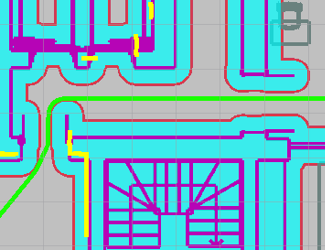
\includegraphics[width=0.98\textwidth, height=5.5cm]{costmap_not_inflated.png}\\
        }
        % {\sourcecitation{Autor}.}
    \end{subfigure}
    \begin{subfigure}{0.5\linewidth}
        {
            \centering
            \caption{Mapa de custo com inflação alta.}
            \label{fig:inflation_high}
            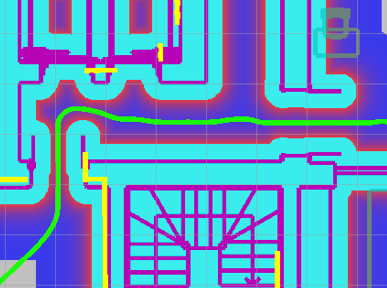
\includegraphics[width=0.98\textwidth, height=5.5cm]{costmap_inflated.png}\\
        }
        % {\sourcecitation{Autor}.}
    \end{subfigure}
\end{figure}

Finalmente, foi testada a camada de obstáculos adicionada neste
trabalho, que utiliza dados da câmera RGB-D para adicionar novos
obstáculos no mapa, mostrado na Figura \ref{fig:voxel_test}. Para
realizar este teste, foi adicionada uma caixa ao mundo do Gazebo,
durante a simulação. Então, foi criada uma rota que passe por este
obstáculo, como na Figura \ref{fig:voxel_before}. Ao se aproximar
desta caixa, ela é detectada pela nuvem de pontos da câmera,
representada como pontos brancos, e é adicionada ao mapa de custom,
como é visto na Figura \ref{fig:voxel_after}.

\begin{figure}[h]
    \caption{Mapeamento de obstáculos da camada \textit{voxel}}
    \label{fig:voxel_test}
    \begin{subfigure}{0.5\linewidth}
        {
            \centering
            \caption{Mapa de custo antes da detecção do obstáculo.}
            \label{fig:voxel_before}
            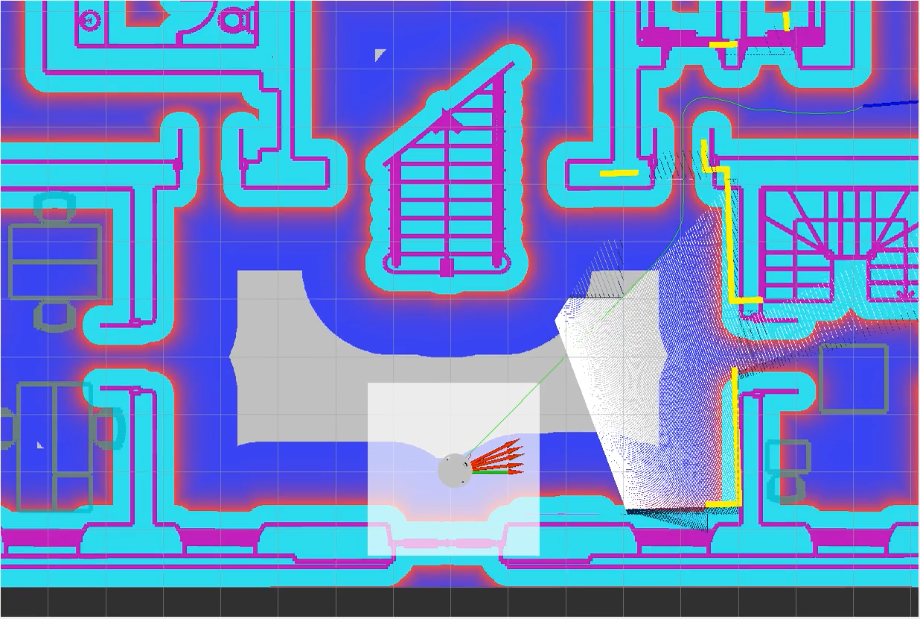
\includegraphics[width=0.98\textwidth]{costmap_voxel_before.png}\\
        }
        % {\sourcecitation{Autor}.}
    \end{subfigure}
    \begin{subfigure}{0.5\linewidth}
        {
            \centering
            \caption{Mapa de custo após a detecção do obstáculo.}
            \label{fig:voxel_after}
            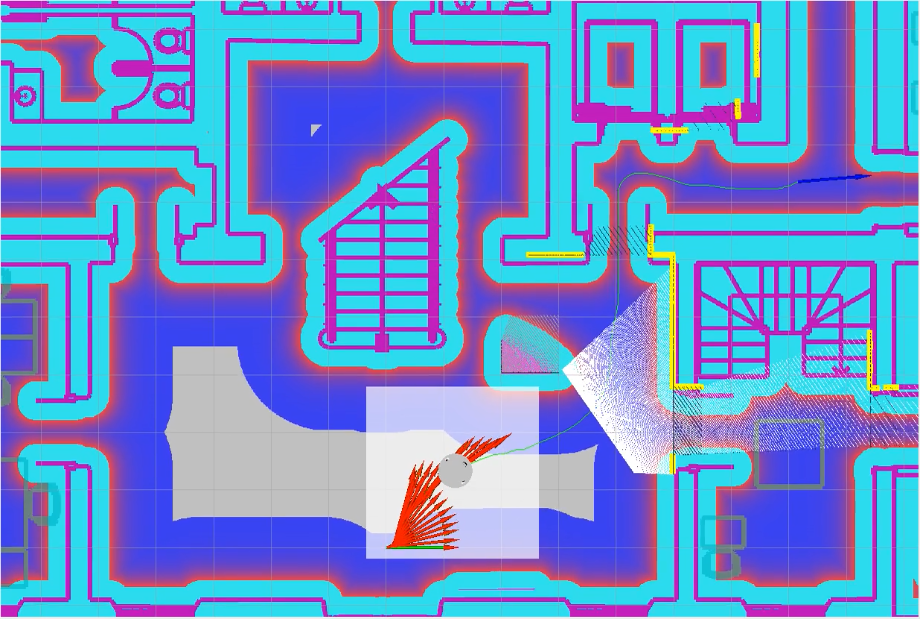
\includegraphics[width=0.98\textwidth]{costmap_voxel_after.png}\\
        }
        % {\sourcecitation{Autor}.}
    \end{subfigure}
\end{figure}

Percebe-se nestas duas imagens, que caso fosse utilizada uma
representação plana do ambiente, na altura da câmera, que pode ser
visto em amarelo nas
Figuras~\ref{fig:voxel_before}~e~\ref{fig:voxel_after}, o obstáculo
não seria detectado, e o robô colidiria com a caixa.

\section{Testes de odometria, localização e mapeamento SLAM}

O testes de odometria, localização e mapeamento SLAM foram realizados
na mesma sacola de dados, como descrito na seção \ref{met:testes},
permitindo dessa forma, a mesma entrada em cada sistema.

Na Figura \ref{fig:base_bag}, é mostrado o robô realizando a
trajetória de testes. As setas em vermelho representam a mensagem de
odometria do robô, onde é indicado a posição e orientação do robô. A
linha verde indica a trajetória planejada do robô. O caminho
realizado neste teste começa na origem, segue em direção a porta no
canto superior direto da sala, percorre o corredor e entra na
primeira sala. É possível comparar a percepção de diferentes
ambientes neste teste, como em corredores estreitos e salas abertas.
A distância total percorrida pelo robô foi de $13,08~\si{\meter}$.

Devido ao tamanho da sacola de dados em razão da captura das imagens
da câmera, não foi possível realizar uma simulação longa, que
percorresse uma grande área do mapa e retornasse ao ponto inicial,
testando assim o fechamento de laço, que é um ponto importante no
mapeamento de sistemas SLAM.

\begin{figure}[h]
    {
        \centering
        \caption{Robô durante o teste realizado.}
        \label{fig:base_bag}
        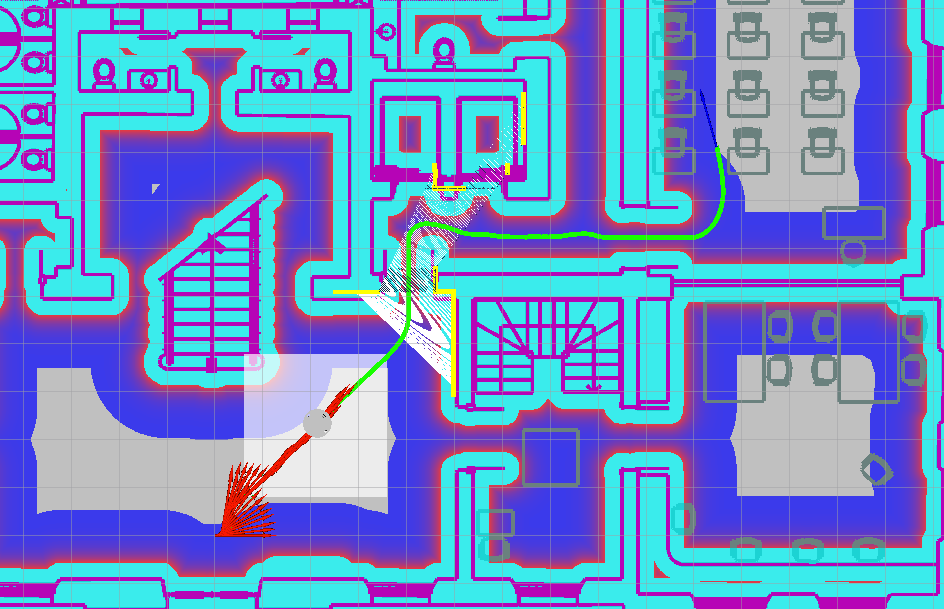
\includegraphics[width=0.95\textwidth]{base_bag_sim_zoom.png}\\
    }
    % {\sourcecitation{Autor}.}
\end{figure}

\subsection{Odometria}

Após o fim da simulação e captura de dados, foram executados os
sistemas de odometria na sacola gerada. Neste teste, utilizou-se a
transformada estática entre os sistemas de coordenadas \texttt{map} e
\texttt{odom}, para comparar a odometria das rodas e visual. A partir
dos dados obtidos, foram criados gráficos com as estimativas da
posição do robô nos eixos X e Y em relação a origem do sistema de
coordenadas \texttt{map} dos sistemas de odometria em verde,
comparados com a posição real do robô em vermelho, e gráficos com o
erro de estimativa de posição ao longo da distância percorrida.

Importante notar que os gráficos de erro de distância apresentam um
ruído aparente, devido a diferença de frequência de publicação das
mensagens de posição real e estimativa de posição. Entre a geração de
uma estimativa e outra, o erro de distância aumenta, já que a posição
real é atualizada e a estimativa não.

A odometria das rodas, mostrada na Figura
\ref{fig:controller_odom_result}, apresentou uma grande divergência
em relação a posição real do robô, com a curva da posição estimada
inclinada para a direita, em relação a curva da posição real, como
mostra a Figura \ref{fig:odom_controller}, indicando um erro na
estimativa da orientação do robô.

O erro de orientação é especialmente indesejado porque, quando é
causado, se transforma em erro de posição lateral e aumenta sem
limite\cite{borenstein}. Na primeira parte do trajeto, da origem até
a primeira porta, a orientação estimada divergiu constantemente,
causando uma curva exponencial do erro, como é visto na Figura
\ref{fig:odom_controller_error}. Este erro continuou crescendo até o
final do trajeto, causando uma grande divergência na posição final,
com uma distância de $6,8~\si{\meter}$ entre a posição real e a
estimada.

\begin{figure}[h]
    \caption{Resultado da odometria das rodas.}
    \label{fig:controller_odom_result}
    \begin{subfigure}{0.5\linewidth}
        {
            \centering
            \caption{Posição estimada da odometria das rodas.}
            \label{fig:odom_controller}
            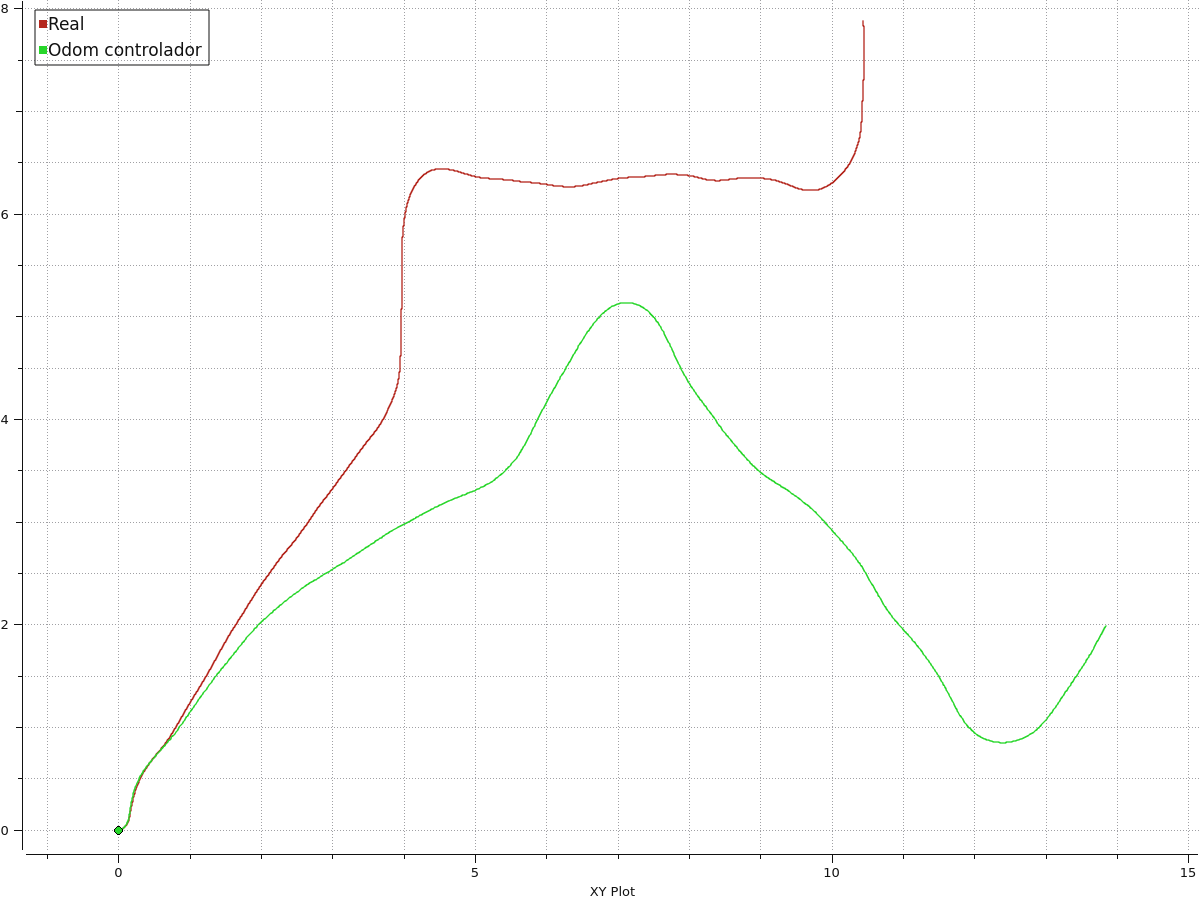
\includegraphics[width=0.98\linewidth]{odom-controlador.png}\\
        }
        % {\sourcecitation{Autor}.}
    \end{subfigure}
    \begin{subfigure}{0.5\linewidth}
        {
            \centering
            \caption{Erro de estimativa da odometria das rodas.}
            \label{fig:odom_controller_error}
            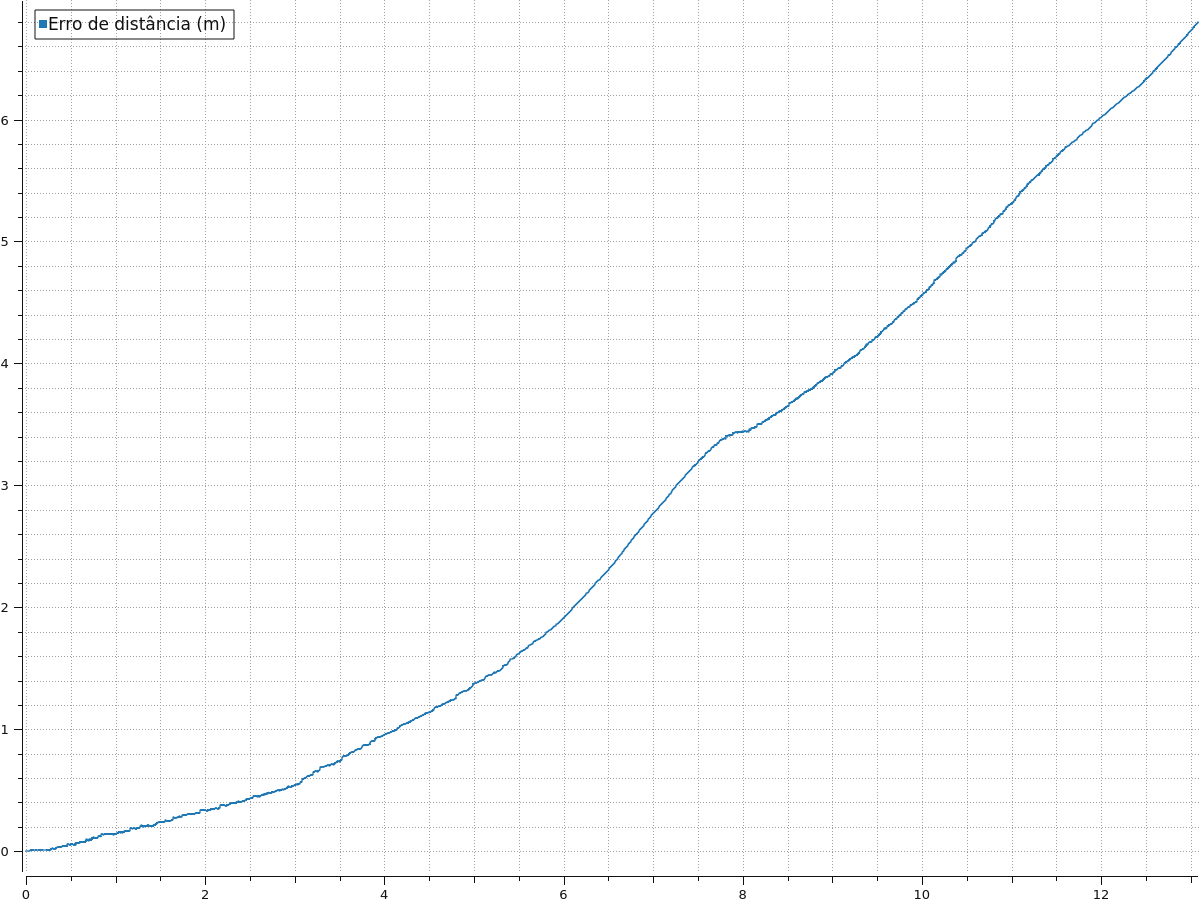
\includegraphics[width=0.98\linewidth]{odom-controlador-error.png}\\
        }
        % {\sourcecitation{Autor}.}
    \end{subfigure}
\end{figure}

Por outro lado, a odometria visual, mostrada na Figura
\ref{fig:visual_odom_result}, apresentou um resultado satisfatório.
No gráfico da posição estimada, da Figura \ref{fig:odom_visual},
mostra que ocorreu a mesma inclinação para a direita que a odometria
das rodas, porém menos acentuada. Como este gráfico não tem
informação sobre o tempo, em certos da trajetória no corredor, a
posição estimada parece estar igual a posição real, porém, na Figura
\ref{fig:odom_visual_error}, é possível perceber que o erro de
estimativa cresceu ao longo deste trajeto, atingindo um erro de
$0,5~\si{\meter}$ no pico. Este erro diminuiu enquanto o robô
percorria a curva final, porém logo aumento novamente atingindo um
erro de $0,66~\si{\meter}$ no final do trajeto.

\begin{figure}[h]
    \caption{Resultado da odometria visual.}
    \label{fig:visual_odom_result}
    \begin{subfigure}{0.5\linewidth}
        {
            \centering
            \caption{Posição estimada da odometria visual.}
            \label{fig:odom_visual}
            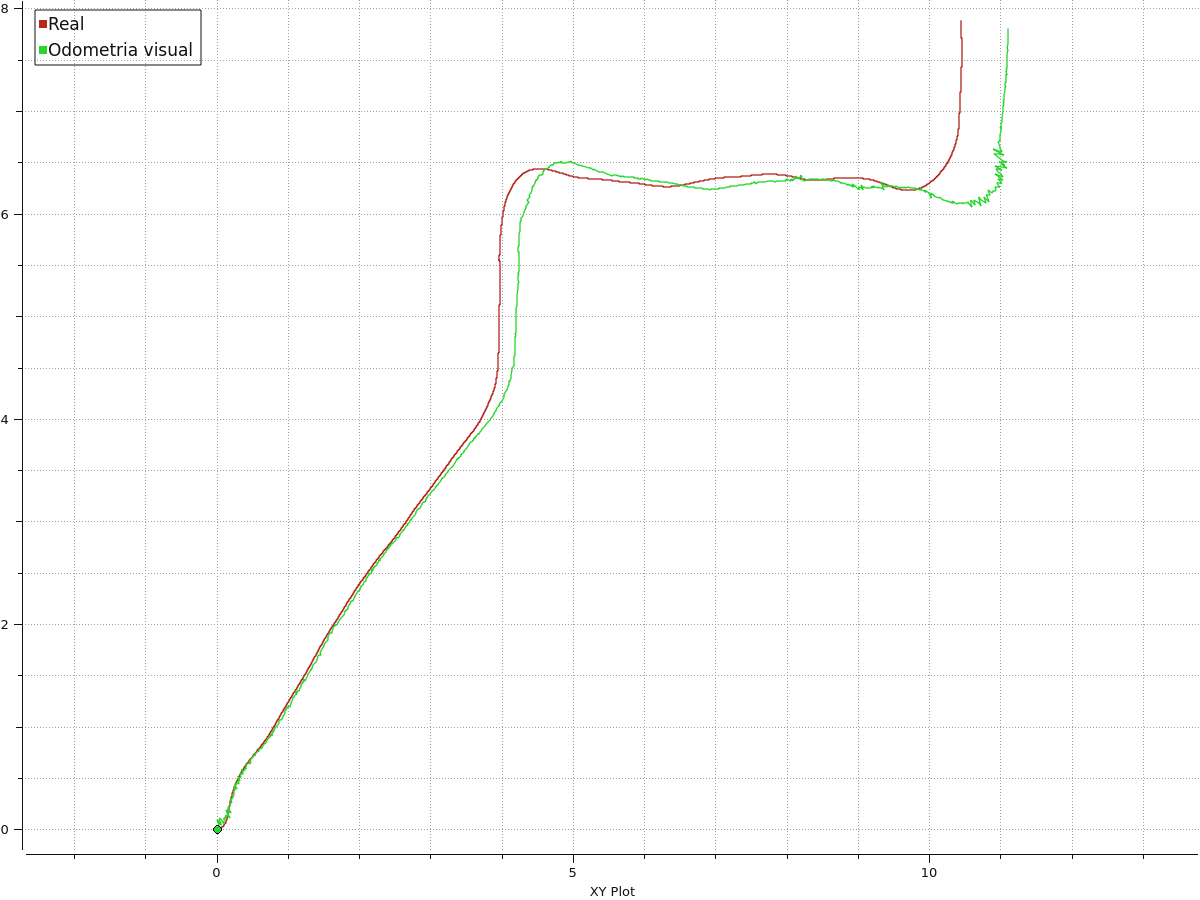
\includegraphics[width=0.98\linewidth]{odom-visual.png}\\
        }
        % {\sourcecitation{Autor}.}
    \end{subfigure}
    \begin{subfigure}{0.5\linewidth}
        {
            \centering
            \caption{Erro de estimativa da odometria visual.}
            \label{fig:odom_visual_error}
            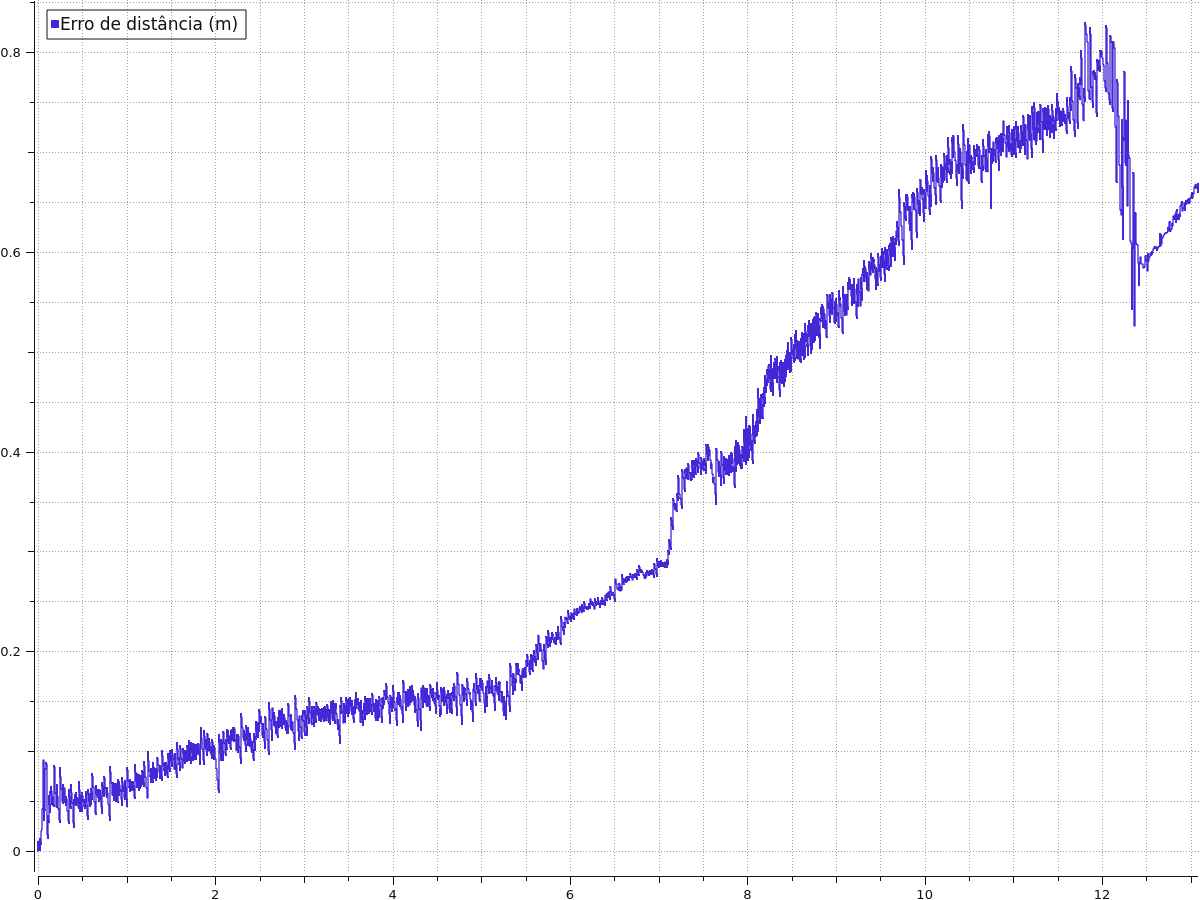
\includegraphics[width=0.98\linewidth]{odom-visual-error.png}\\
        }
        % {\sourcecitation{Autor}.}
    \end{subfigure}
\end{figure}

\subsection{Localização}

Como a odometria visual apresentou um resultado satisfatório, ela foi
utilizada em conjunto com os sistemas de localização, onde será
testado o ajuste dos erros de odometria pelo sistema de localização.
Portanto, foram criados novos gráficos, adicionando a posição global
estimada pelos sistemas de localização, em azul. Esta posição é
obtida através da transformada entre \texttt{map}, \texttt{odom} e
\texttt{base\_link}.

A Figura \ref{fig:rtabmap_slam_result} mostra o resultado do sistema
de localização do pacote \texttt{rtabmap\_slam}. A localização neste
caso teve um ajuste bem pequeno, diminuindo o erro para
$0,63~\si{\meter}$ no pico na posição final. É possível perceber pelo
gráfico da Figura \ref{fig:localization_rtabmap_error} que a curva do
erro manteve uma forma semelhante a curva do erro da odometria
visual. Porém, houve menos ruído na estimativa de posição, como
mostra a Figura \ref{fig:localization_rtabmap}.

\begin{figure}[h]
    \caption{Resultado do pacote \texttt{rtabmap\_slam}.}
    \label{fig:rtabmap_slam_result}
    \begin{subfigure}{0.5\linewidth}
        {
            \centering
            \caption{Posição estimada do \texttt{rtabmap\_slam}.}
            \label{fig:localization_rtabmap}
            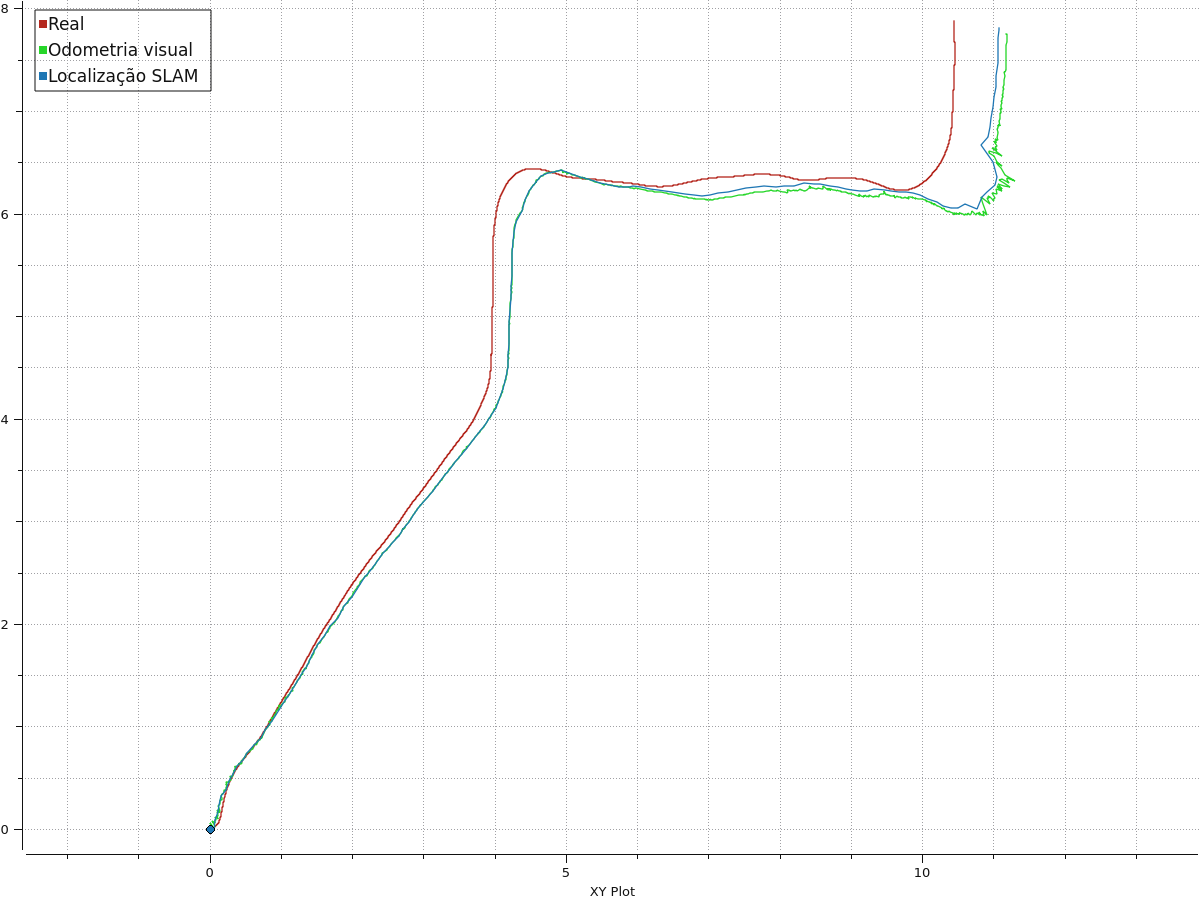
\includegraphics[width=0.98\linewidth]{localization-rtabmap.png}\\
        }
        % {\sourcecitation{Autor}.}
    \end{subfigure}
    \begin{subfigure}{0.5\linewidth}
        {
            \centering
            \caption{Erro de estimativa do \texttt{rtabmap\_slam}.}
            \label{fig:localization_rtabmap_error}
            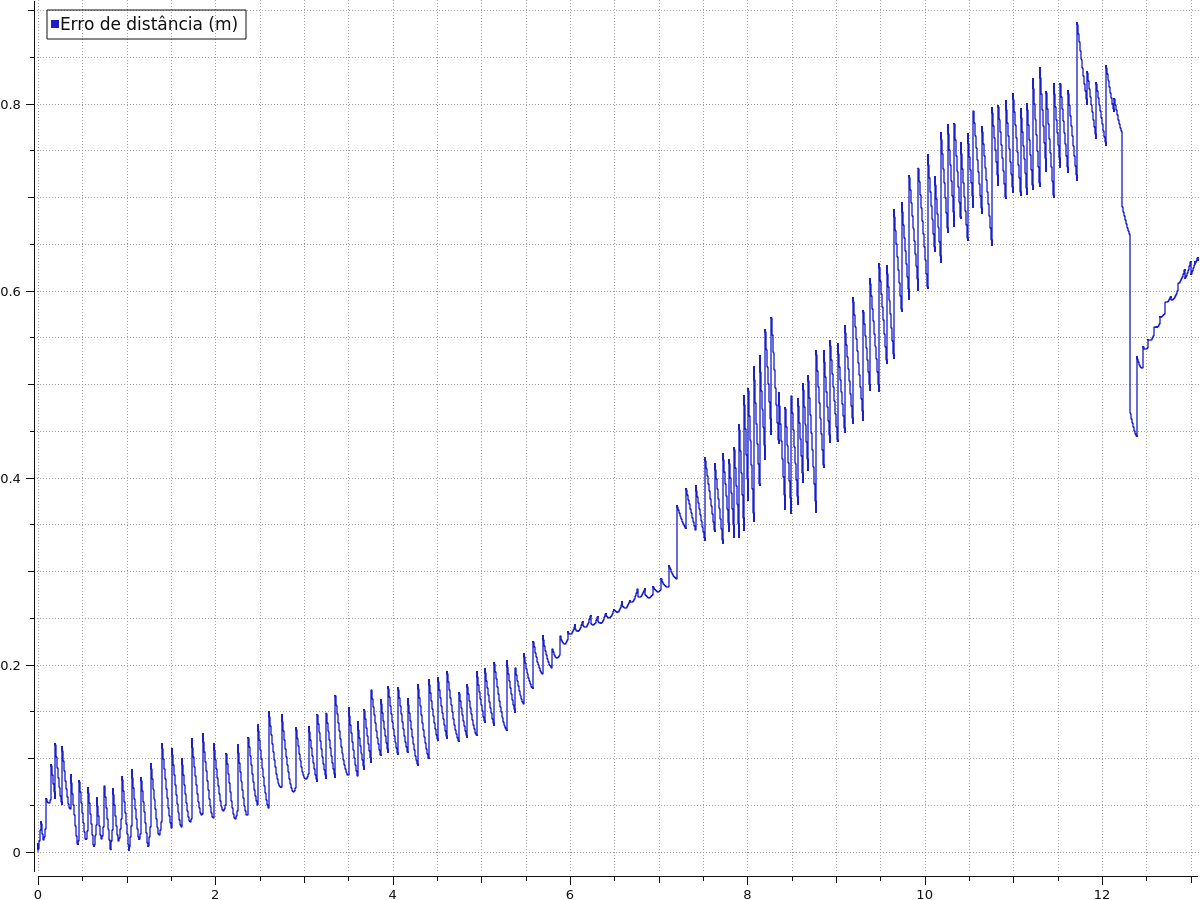
\includegraphics[width=0.98\linewidth]{localization-rtabmap-error.png}\\
        }
        % {\sourcecitation{Autor}.}
    \end{subfigure}
\end{figure}

O \texttt{slam\_toolbox}, que têm seu resultado representado na
Figura \ref{fig:slam_toolbox_result}, por outro lado, apresentou um
resultado melhor, diminuindo o erro de estimativa para
aproximadamente $0,37~\si{\meter}$ no final da trajetória. Isto
aconteceu em grande parte porque não houve o acumulo de erro durante
o trajeto do corredor, como mostra a Figura
\ref{fig:localization_slam_toolbox_error}, que havia acontecido na
odometria visual. A Figura \ref{fig:localization_slam_toolbox} mostra
que o ruído na estimativa de posição foi atenuado da mesma forma que
o \texttt{rtabmap\_slam}.

\begin{figure}[h]
    \caption{Resultado do pacote \texttt{slam\_toolbox}.}
    \label{fig:slam_toolbox_result}
    \begin{subfigure}{0.5\linewidth}
        {
            \centering
            \caption{Posição estimada do \texttt{slam\_toolbox}.}
            \label{fig:localization_slam_toolbox}
            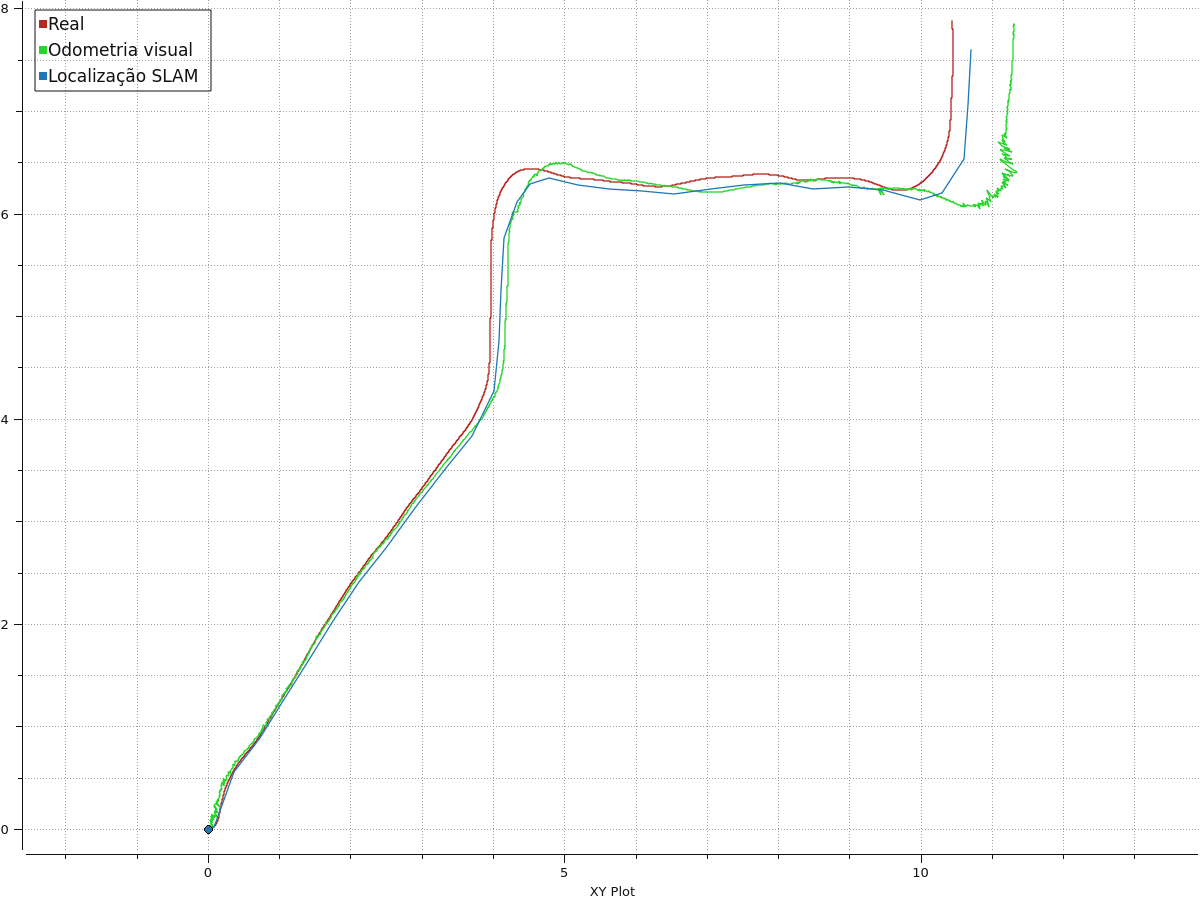
\includegraphics[width=0.98\linewidth]{localization-slam-toolbox.png}\\
        }
        % {\sourcecitation{Autor}.}
    \end{subfigure}
    \begin{subfigure}{0.5\linewidth}
        {
            \centering
            \caption{Erro de estimativa do \texttt{slam\_toolbox}.}
            \label{fig:localization_slam_toolbox_error}
            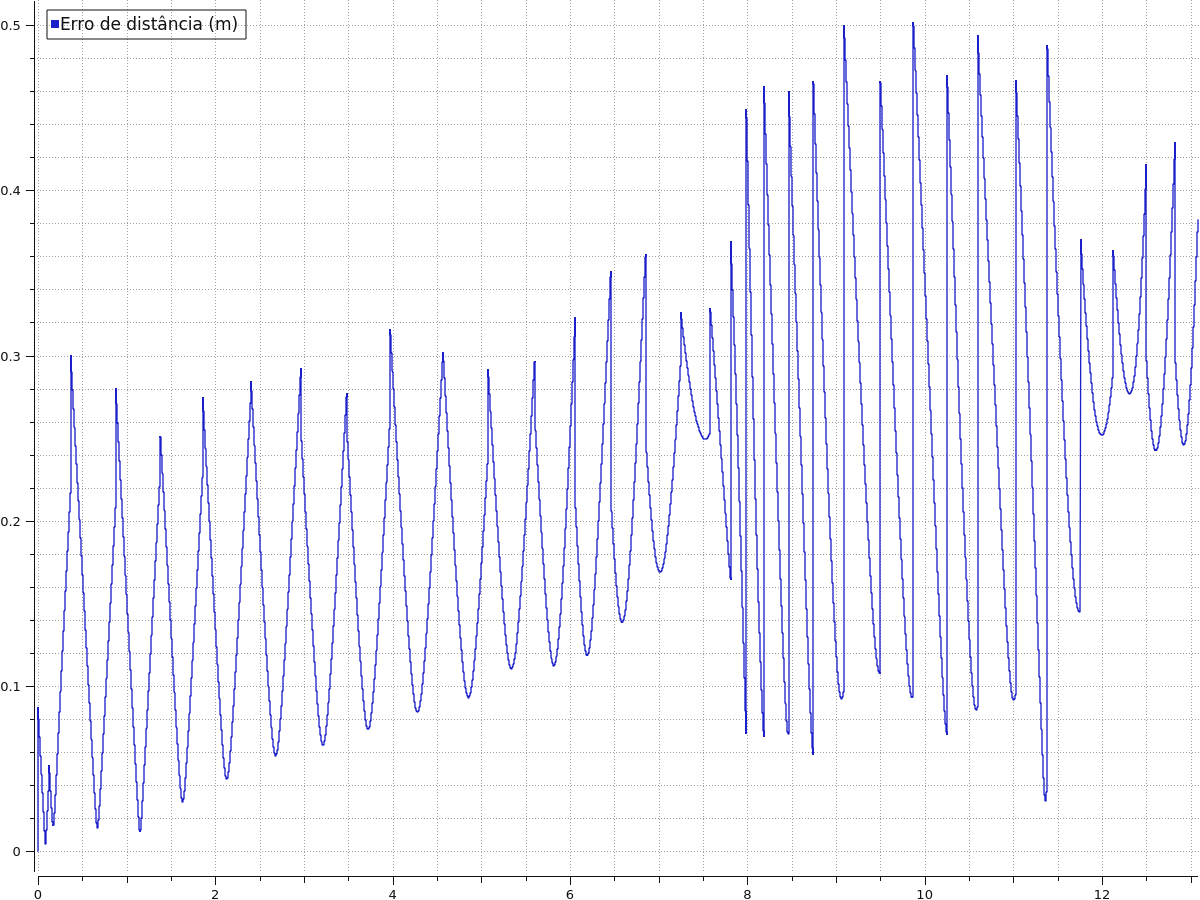
\includegraphics[width=0.98\linewidth]{localization-slam-toolbox-error.png}\\
        }
        % {\sourcecitation{Autor}.}
    \end{subfigure}
\end{figure}

Nota-se que, apesar de utilizar a mesma entrada em todas execuções da
simulação, a odometria visual apresentou resultados ligeiramente
diferentes em cada execução. Isto acontece porque a máquina utilizada
para a execução não possui capacidade de processamento suficiente
para realizar os cálculos necessários por estes pacotes na frequência
configurada. Na execução com o texttt{slam\_toolbox}, que exige alta
capacidade de processamento, este problema foi mais evidente. Os
algoritmos de SLAM também sofreram este problema. Portanto, em
máquinas mais potentes, a estimativa de posição pode ser mais
precisa.

\subsection{Mapeamento SLAM}

Como mencionado anteriormente, os dois sistemas de localização
utilizados realizam o mapeamento simultaneamente com a localização.
Portanto, tanto o \texttt{slam\_toolbox} quanto o
\texttt{rtabmap\_slam} geraram um mapa do ambiente durante a execução
da simulação. Estes mapas podem ser utilizados para novas sessões de
localização, ou em mapas de custo para planejamento de trajetória.

Na Figura \ref{fig:mapping_rtabmap}, é mostrado o mapa gerado pelo
\texttt{rtabmap\_slam}, que cria um mapa utilizando os dados
tridimensionais da câmera RGB-D, enquanto que na Figura
\ref{fig:mapping_slam_toolbox} é mostrado o mapa gerado pelo
\texttt{slam\_toolbox}, que utiliza uma conversão da imagem de
profundidade em um feixe de luz em duas dimensões. A representação do
ambiente no Gazebo foi sobreposta aos mapas para facilitar a
comparação. Nestes mapas, as áreas em branco claro são áreas livres,
e as áreas em preto são consideradas ocupadas, enquanto que as áreas
em cinza são desconhecidas.

\begin{figure}[h]
    {
        \centering
        \caption{Mapa construído pelo \texttt{rtabmap\_slam}.}
        \label{fig:mapping_rtabmap}
        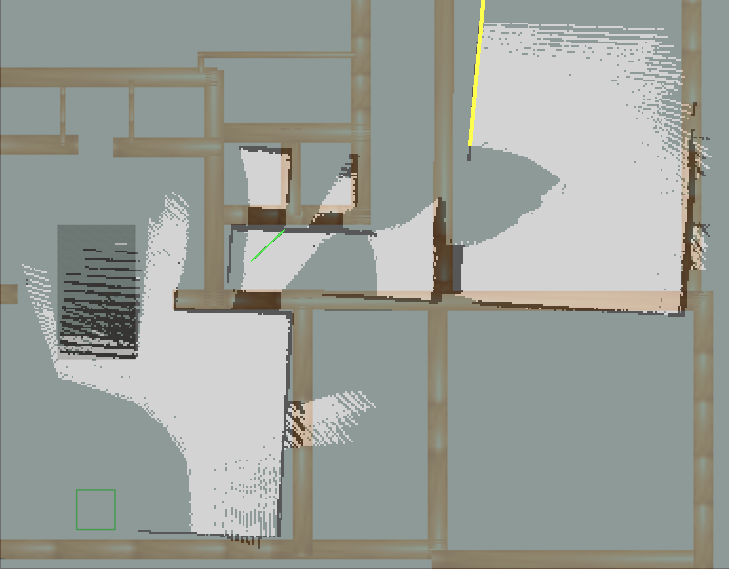
\includegraphics[width=0.8\linewidth]{rtabmap_slam_map-compared.png}\\
    }
    % {\sourcecitation{Autor}.}
\end{figure}

\begin{figure}[htbp]
    {
        \centering
        \caption{Mapa construído pelo \texttt{slam\_toolbox}.}
        \label{fig:mapping_slam_toolbox}
        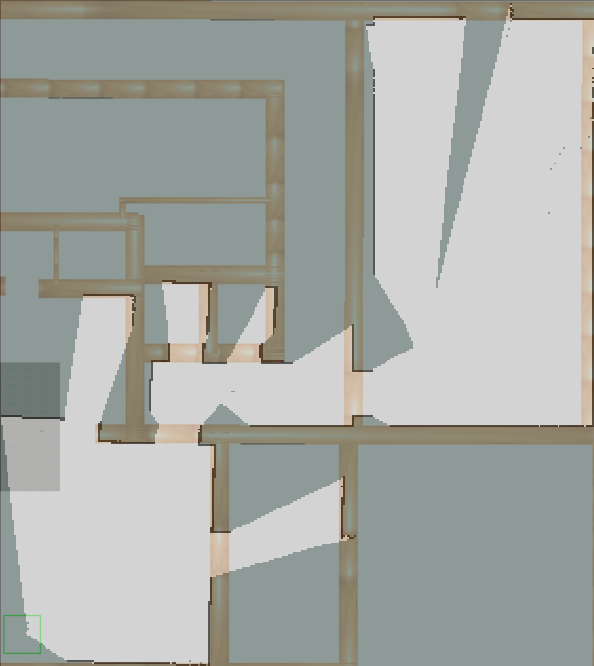
\includegraphics[width=0.6\linewidth]{slam_toolbox_map-compared.png}\\
    }
    % {\sourcecitation{Autor}.}
\end{figure}

É possível perceber diferenças na geração destes mapas devido ao tipo de mensagem
utilizado. O mapa gerado pelo \texttt{rtabmap\_slam} gera um representação mais
detalhada da escada, percebendo-a desde sua base, enquanto que o \texttt{slam\_toolbox}
só mapeia a escada na mesma altura da câmera, que é a altura da mensagem passada
a ela.
Além disso, o \texttt{rtabmap\_slam} mapeou as molduras das portas, que estão acima
da altura da câmera. Este comportamento, porém, pode ser modificado, já que
não são obstáculos relevantes para a navegação.

Outro diferença é no mapeamento do chão dos mapas. Devido ao campo de
visão da câmera, não é captado o chão em frente ao robô, que portanto
não é mapeado pelo \texttt{rtabmap\_slam}. Por outro lado, como o
\texttt{slam\_toolbox} utiliza um feixe de luz em duas dimensões, é
considerado que todo espaço entre o robô e o primeiro obstáculo
detectado é livre, mapeando assim o chão não captado pela câmera. Em
situações em que não é detectado nenhum obstáculo dentro do limite da
câmera, como a área entre o final da trajetória do robô e a porta da
sala no canto superior direito da Figura
\ref{fig:mapping_slam_toolbox}, o chão não é mapeado.

Percebe-se, também, que o mapa gerado pelo \texttt{slam\_toolbox} é
mais fiel quanto a posição das paredes do ambiente real, já que o
mapa gerado pelo \texttt{rtabmap\_slam} possui uma inclinação que não
corresponde ao ambiente real. Isto é devido a estimativa da posição
do robô, apresentadas anteriormente, em que o \texttt{slam\_toolbox}
apresentou uma estimativa mais precisa.

\chapter{Discussão}
\label{discussao}

Os resultados obtidos demonstram que a utilização da câmera no robô
Twil permite o mapeamento do ambiente em tempo-real, possibilitando a
navegação autônoma do robô em ambientes desconhecidos ou com
obstáculos dinâmicos. Isto foi realizado através da atualização do
mapa de custos utilizado pelo planejador de trajetórias. Com uma
camada \textit{voxel}, responsável por detectar obstáculos
tridimensionais no ambiente, e uma camada de inflação, que cria uma
zona de segurança ao redor dos obstáculos, o robô é capaz de evitar
colisões. Este sistema pode ser aprimorado com a utilização de outras
camadas do mapa de custo, como a camada \textit{Spatio Temporal Voxel
    Layer}~\cite{stlv_article}, que adiciona um decaimento temporal ao
obstáculos detectados, já que eles podem ser temporários.

Além disso, a câmera aprimorou a estimativa de posição do robô, que
permite o seguimento correto da trajetória planejada. A combinação de
odometria e localização que produziu a melhor estimativa foi a
odometria visual, utilizando o pacote \texttt{rtabmap\_odom} com a
localização do pacote \texttt{slam\_toolbox}.

A escolha da odometria se da pelo desempenho superior da odometria
visual em relação a odometria das rodas. Porém, a odometria das rodas
apresentou um resultado pior do que o esperado, podendo ser causado
por erros na descrição do robô, o que pode ser ajustado. Além disso,
a odometria visual pode apresentar resultados inferiores em ambientes
reais, devido ao maior ruído presente fora da simulação, que foi
feita em condições ideias.

Logo, em trabalhos futuros, recomenda-se ajustes no sistema de
odometria das rodas, para garantir uma estimativa mais precisa da
posição do robô. Como discutido anteriormente, a odometria das rodas
apresentou um erro substantivo na estimada de odometria, que é o erro
mais preocupante da odometria. Para mitigar este erro, é possível
utilizar as informações de velocidade angular e orientação do IMU
presente no robô para calcular a estimativa de posição.

Isto pode ser feito utilizando o pacote \texttt{robot\_localization},
retirando a utilização de dados da posição dada pela mensagem
publicada pela odometria das rodas. Desta forma, a posição do robô
seria calculada utilizando a velocidade linear das rodas e a
orientação do IMU, obtendo assim uma estimativa com menor erro.
Porém, a velocidade publicada pela odometria das rodas deve ser
modificada para ser em relação a base do robô, como é esperado pelo
\texttt{robot\_localization}, e não em relação ao sistema de
coordenadas \texttt{odom}, como é publicada atualmente.

Com a odometria das rodas ajustada, ambos sistemas de odometria devem
ser comparados novamente. Em caso de desempenho semelhante,
recomenda-se a utilização da odometria das rodas, por ser mais
simples exigindo menor capacidade de computacional. Porém, caso a
complexidade de processamento não seja um problema, ambas odometria
podem ser utilizadas em conjunto, fundidas através de um filtro de
Kalman para obter uma estimativa mais precisa da posição do robô.

Em relação ao mapeamento, o pacote \texttt{rtabmap\_slam} criou um
mapa mais detalhado do ambiente, devido a utilização de dados
tridimensionais. Porém, isto não afetou o desempenho da navegação,
com o \texttt{slam\_toolbox} apresentando uma melhor estimativa de
posição. Portanto, caso seja desejado um mapa do ambiente mais
detalhado, recomenda-se a utilização do \texttt{rtabmap\_slam}, em
uma sacola de dados, e não durante a navegação em tempo-real, da
mesma forma que foi feito neste trabalho.

Além disso, devem ser realizados testes de SLAM que percorram um
caminho que revisite áreas já vistas, para testar o fechamento de
laço. Não foi possível testar isto neste trabalho, porque a execução
da simulação em conjunto com os sistemas de odometria e localização
exigiu muita capacidade de processamento, e as sacolas de dados, que
permitem separar a execução destes sistemas, não são praticáveis em
trajetórias longas, devido ao tamanho do arquivo gerado.

\chapter{Conclusão}
\label{conclusao}

Este trabalho atingiu o objetivo proposto de mapear o ambiente para
navegação autônoma utilizando a câmera RGB-D do robô Twil, evitando
assim colisões em ambientes dinâmicos ou pouco conhecidos. Porém, os
testes foram realizados apenas em ambiente simulado, já que o sistema
não foi implementado no robô real. Em trabalhos futuros, o
desenvolvimento deste trabalho pode ser aplicado no robô real. Para
isso, o Gazebo deverá ser dispensado e os dados deverão todos ser
obtidos através do robô real. Porém, primeiramente deve ser realizado
os ajustes na odometria das rodas, detalhado na discussão deste
trabalho. Ao implementar o sistema no robô real, é possível que seja
necessária uma recalibração dos sistemas de odometria e localização.
Neste caso, recomenda-se a utilização dos programas de gravação de
sacolas utilizados neste trabalho para análise dos resultados, já que
não deve existir diferença entre os tópicos publicados pelo robô real
e pela simulação.

\printbibliography

%\begin{appendix}
%
%\end{appendix}
%
%
%\begin{annex}
%\end{annex}

\end{document}

